%%%%%%%%%%%%%%%%%%%%%%%%%%%%%%%%%%%%%%%%%
%  My documentation report
%  Objetive: Explain what I did and how, so someone can continue with the investigation
%
% Important note:
% Chapter heading images should have a 2:1 width:height ratio,
% e.g. 920px width and 460px height.
%
%%%%%%%%%%%%%%%%%%%%%%%%%%%%%%%%%%%%%%%%%

%----------------------------------------------------------------------------------------
%	PACKAGES AND OTHER DOCUMENT CONFIGURATIONS
%----------------------------------------------------------------------------------------

\documentclass[11pt,fleqn]{book} % Default font size and left-justified equations

\usepackage[top=3cm,bottom=3cm,left=3.2cm,right=3.2cm,headsep=10pt,letterpaper]{geometry} % Page margins
\usepackage[dvipsnames]{xcolor}
\usepackage{lipsum} % Required for specifying colors by name

% Font Settings
\usepackage{avant} % Use the Avantgarde font for headings
%\usepackage{times} % Use the Times font for headings
\usepackage{mathptmx} % Use the Adobe Times Roman as the default text font together with math symbols from the Symbol, Chancery and Computer Modern fonts

\usepackage{microtype} % Slightly tweak font spacing for aesthetics
\usepackage[utf8]{inputenc} % Required for including letters with accents
\usepackage[T1]{fontenc} % Use 8-bit encoding that has 256 glyphs

%-------- LANGUAGE ------
\usepackage{ifthen}

\provideboolean{lfrench}\setboolean{lfrench}{false} 
\provideboolean{lenglish}\setboolean{lenglish}{false} 

%\setboolean{lfrench}{true} 
\setboolean{lenglish}{true}

\ifthenelse{\boolean{lfrench}}{
\usepackage[french]{varioref}
\usepackage[french]{babel}
}{}

\ifthenelse{\boolean{lenglish}}{
\usepackage[english]{varioref}
\usepackage[english]{babel}
}{}

% ------------------
\usepackage{wrapfig}
\usepackage{listings}
\usepackage{multicol}
\usepackage{multirow}
\usepackage{colortbl}
\usepackage{booktabs}
\newcommand{\tabitem}{~~\llap{\textbullet}~~}
\usepackage{hyperref}
\usepackage{qrcode}
\usepackage{soul}
\usepackage{tabto}
\usepackage{multienum}


\definecolor{deepblue}{rgb}{0.0,0.0,0.5}
\definecolor{deepred}{rgb}{0.6,0,0}
\definecolor{deepgreen}{rgb}{0,0.5,0}
\definecolor{ocre}{RGB}{51,102,0} 
\definecolor{lightgray}{RGB}{229,229,229} 
\definecolor{palerod}{RGB}{238,232,170}
\definecolor{verttelecom}{RGB}{171,180,0}

\newcommand\pythonstyle{\lstset{
language=Python,
basicstyle=\ttfamily\footnotesize,
morekeywords={self},              % Add keywords here
frame=tb,                         % Any extra options here
showstringspaces=false
}}

\definecolor{backcolour}{rgb}{0.95,0.95,0.92}

\newcommand\termctyle{\lstset{
frame=tb,                         % Any extra options here
showstringspaces=false
}}


% Python environment
\lstnewenvironment{python}[1][]
{
\pythonstyle
\lstset{#1}
}
{}

\lstnewenvironment{termc}[1][]
{
\lstset{#1}
}
{}


% RFC
\newcommand\rfc[1]{\href{http://www.ietf.org/rfc/rfc#1.txt}{\textcolor{blue}{RFC #1}\index{RFC #1}}}
\newcommand\pfunction[2]{\texttt{#2}\index{Module Python!#1!#2}}

% boot.py

\newcommand\glos[1]{\gls{#1}\index{#1}}
\newcommand\pprog[2]{\href{https://github.com/ltn22/PLIDObis/blob/master/#2/#1}{\texttt{#1}}\index{Programmes Python!#1}}
\newcommand\lprog[2]{\href{https://github.com/ltn22/PLIDObis/blob/master/#2/#1}{\texttt{#1}}\index{Programmes micro-python!#1}}

% QUESTION

\usepackage[most]{tcolorbox}

\provideboolean{Response}\setboolean{Response}{true}

\newcommand{\Correct}[1]{\ifthenelse{\boolean{Response}}{#1}{\textbf{#1}}}
\newcommand{\Wrong}[1]{\ifthenelse{\boolean{Response}}{#1}{\textcolor{black!20}{#1}}}

\newwrite\tempfile
\immediate\openout\tempfile=questions.tex


\newtcbtheorem[auto counter,number within=section]{theo}%
  {Question}{fonttitle=\bfseries\upshape, 
     arc=0mm, colback=blue!5!white,colframe=blue!75!black}{Question}
     
\newcommand\Question[3]{
\begin{theo}{#1}{summation}
#2
\immediate\write\tempfile{\noexpand\textbf{Question \thetcbcounter {} page \thepage} {} }
\immediate\write\tempfile{\unexpanded{#2}\noexpand\vspace{1em}\noexpand\newline}
\immediate\write\tempfile{\unexpanded{#3}\noexpand\newline\noexpand\newline}

\end{theo}
}

% MATHS PACKAGE
\usepackage{amsmath,tikz}
\usetikzlibrary{matrix}
\newcommand*{\horzbar}{\rule[0.05ex]{2.5ex}{0.5pt}}
\usepackage{calc}

% VERBATIM PACKAGE
\usepackage{verbatim}

\usepackage{tikz}

\usetikzlibrary{automata}
\usetikzlibrary[shadows]
\usetikzlibrary{shapes}
\usetikzlibrary[decorations.footprints] 
\usetikzlibrary{decorations.pathmorphing}
\usetikzlibrary{decorations.pathreplacing}
\usetikzlibrary{decorations.text}
\usetikzlibrary {arrows}
\usetikzlibrary{patterns}
\usetikzlibrary{calc}
\usetikzlibrary{external}

\usepackage{tikz-timing}

% Acronyms

\usepackage{makeidx}
\makeindex

\usepackage{acronym}

\let\oldac\ac
\renewcommand*{\ac}[1]{\oldac{#1}\index{#1}}

\newcommand\Index[1]{\textbf{#1}\index{#1}}

% Bibliography
\usepackage[style=alphabetic,sorting=nyt,sortcites=true,autopunct=true,babel=hyphen,hyperref=true,abbreviate=false,backref=true,backend=biber]{biblatex}
\addbibresource{bibliography.bib} % BibTeX bibliography file
\defbibheading{bibempty}{}

%----------------------------------------------------------------------------------------
%	VARIOUS REQUIRED PACKAGES
%----------------------------------------------------------------------------------------

\usepackage{titlesec} % Allows customization of titles

\usepackage{graphicx} % Required for including pictures
\graphicspath{{Pictures/}} % Specifies the directory where pictures are stored

\usepackage{lipsum} % Inserts dummy text

\usepackage{tikz} % Required for drawing custom shapes

\usepackage[french]{babel} % English language/hyphenation

\usepackage{enumitem} % Customize lists
\setlist{nolistsep} % Reduce spacing between bullet points and numbered lists

\usepackage{booktabs} % Required for nicer horizontal rules in tables

\usepackage{eso-pic} % Required for specifying an image background in the title page

%----------------------------------------------------------------------------------------
%	MAIN TABLE OF CONTENTS
%----------------------------------------------------------------------------------------

\usepackage{titletoc} % Required for manipulating the table of contents

\contentsmargin{0cm} % Removes the default margin
% Chapter text styling
\titlecontents{chapter}[1.25cm] % Indentation
{\addvspace{15pt}\large\sffamily\bfseries} % Spacing and font options for chapters
{\color{ocre!60}\contentslabel[\Large\thecontentslabel]{1.25cm}\color{ocre}} % Chapter number
{}  
{\color{ocre!60}\normalsize\sffamily\bfseries\;\titlerule*[.5pc]{.}\;\thecontentspage} % Page number
% Section text styling
\titlecontents{section}[1.25cm] % Indentation
{\addvspace{5pt}\sffamily\bfseries} % Spacing and font options for sections
{\contentslabel[\thecontentslabel]{1.25cm}} % Section number
{}
{\sffamily\hfill\color{black}\thecontentspage} % Page number
[]
% Subsection text styling
\titlecontents{subsection}[1.25cm] % Indentation
{\addvspace{1pt}\sffamily\small} % Spacing and font options for subsections
{\contentslabel[\thecontentslabel]{1.25cm}} % Subsection number
{}
{\sffamily\;\titlerule*[.5pc]{.}\;\thecontentspage} % Page number
[] 

%----------------------------------------------------------------------------------------
%	MINI TABLE OF CONTENTS IN CHAPTER HEADS
%----------------------------------------------------------------------------------------

% Section text styling
\titlecontents{lsection}[0em] % Indendating
{\footnotesize\sffamily} % Font settings
{}
{}
{}

% Subsection text styling
\titlecontents{lsubsection}[.5em] % Indentation
{\normalfont\footnotesize\sffamily} % Font settings
{}
{}
{}
 
%----------------------------------------------------------------------------------------
%	PAGE HEADERS
%----------------------------------------------------------------------------------------

\usepackage{fancyhdr} % Required for header and footer configuration

\pagestyle{fancy}
\renewcommand{\chaptermark}[1]{\markboth{\sffamily\normalsize\bfseries\chaptername\ \thechapter.\ #1}{}} % Chapter text font settings
\renewcommand{\sectionmark}[1]{\markright{\sffamily\normalsize\thesection\hspace{5pt}#1}{}} % Section text font settings
\fancyhf{} \fancyhead[LE,RO]{\sffamily\normalsize\thepage} % Font setting for the page number in the header
\fancyhead[LO]{\rightmark} % Print the nearest section name on the left side of odd pages
\fancyhead[RE]{\leftmark} % Print the current chapter name on the right side of even pages
\renewcommand{\headrulewidth}{0.5pt} % Width of the rule under the header
\addtolength{\headheight}{2.5pt} % Increase the spacing around the header slightly
\renewcommand{\footrulewidth}{0pt} % Removes the rule in the footer
\fancypagestyle{plain}{\fancyhead{}\renewcommand{\headrulewidth}{0pt}} % Style for when a plain pagestyle is specified

% Removes the header from odd empty pages at the end of chapters
\makeatletter
\renewcommand{\cleardoublepage}{
\clearpage\ifodd\c@page\else
\hbox{}
\vspace*{\fill}
\thispagestyle{empty}
\newpage
\fi}

%----------------------------------------------------------------------------------------
%	THEOREM STYLES
%----------------------------------------------------------------------------------------

\usepackage{amsmath,amsfonts,amssymb,amsthm} % For math equations, theorems, symbols, etc

\newcommand{\intoo}[2]{\mathopen{]}#1\,;#2\mathclose{[}}
\newcommand{\ud}{\mathop{\mathrm{{}d}}\mathopen{}}
\newcommand{\intff}[2]{\mathopen{[}#1\,;#2\mathclose{]}}
\newtheorem{notation}{Notation}[chapter]

%%%%%%%%%%%%%%%%%%%%%%%%%%%%%%%%%%%%%%%%%%%%%%%%%%%%%%%%%%%%%%%%%%%%%%%%%%%
%%%%%%%%%%%%%%%%%%%% dedicated to boxed/framed environements %%%%%%%%%%%%%%
%%%%%%%%%%%%%%%%%%%%%%%%%%%%%%%%%%%%%%%%%%%%%%%%%%%%%%%%%%%%%%%%%%%%%%%%%%%
\newtheoremstyle{ocrenumbox}% % Theorem style name
{0pt}% Space above
{0pt}% Space below
{\normalfont}% % Body font
{}% Indent amount
{\small\bf\sffamily\color{ocre}}% % Theorem head font
{\;}% Punctuation after theorem head
{0.25em}% Space after theorem head
{\small\sffamily\color{ocre}\thmname{#1}\nobreakspace\thmnumber{\@ifnotempty{#1}{}\@upn{#2}}% Theorem text (e.g. Theorem 2.1)
\thmnote{\nobreakspace\the\thm@notefont\sffamily\bfseries\color{black}---\nobreakspace#3.}} % Optional theorem note
\renewcommand{\qedsymbol}{$\blacksquare$}% Optional qed square

\newtheoremstyle{blacknumex}% Theorem style name
{5pt}% Space above
{5pt}% Space below
{\normalfont}% Body font
{} % Indent amount
{\small\bf\sffamily}% Theorem head font
{\;}% Punctuation after theorem head
{0.25em}% Space after theorem head
{\small\sffamily{\tiny\ensuremath{\blacksquare}}\nobreakspace\thmname{#1}\nobreakspace\thmnumber{\@ifnotempty{#1}{}\@upn{#2}}% Theorem text (e.g. Theorem 2.1)
\thmnote{\nobreakspace\the\thm@notefont\sffamily\bfseries---\nobreakspace#3.}}% Optional theorem note

\newtheoremstyle{blacknumbox} % Theorem style name
{0pt}% Space above
{0pt}% Space below
{\normalfont}% Body font
{}% Indent amount
{\small\bf\sffamily}% Theorem head font
{\;}% Punctuation after theorem head
{0.25em}% Space after theorem head
{\small\sffamily\thmname{#1}\nobreakspace\thmnumber{\@ifnotempty{#1}{}\@upn{#2}}% Theorem text (e.g. Theorem 2.1)
\thmnote{\nobreakspace\the\thm@notefont\sffamily\bfseries---\nobreakspace#3.}}% Optional theorem note

%%%%%%%%%%%%%%%%%%%%%%%%%%%%%%%%%%%%%%%%%%%%%%%%%%%%%%%%%%%%%%%%%%%%%%%%%%%
%%%%%%%%%%%%% dedicated to non-boxed/non-framed environements %%%%%%%%%%%%%
%%%%%%%%%%%%%%%%%%%%%%%%%%%%%%%%%%%%%%%%%%%%%%%%%%%%%%%%%%%%%%%%%%%%%%%%%%%
\newtheoremstyle{ocrenum}% % Theorem style name
{5pt}% Space above
{5pt}% Space below
{\normalfont}% % Body font
{}% Indent amount
{\small\bf\sffamily\color{ocre}}% % Theorem head font
{\;}% Punctuation after theorem head
{0.25em}% Space after theorem head
{\small\sffamily\color{ocre}\thmname{#1}\nobreakspace\thmnumber{\@ifnotempty{#1}{}\@upn{#2}}% Theorem text (e.g. Theorem 2.1)
\thmnote{\nobreakspace\the\thm@notefont\sffamily\bfseries\color{black}---\nobreakspace#3.}} % Optional theorem note
\renewcommand{\qedsymbol}{$\blacksquare$}% Optional qed square
\makeatother

% Defines the theorem text style for each type of theorem to one of the three styles above
\newcounter{dummy} 
\numberwithin{dummy}{section}
\theoremstyle{ocrenumbox}
\newtheorem{theoremeT}[dummy]{Theorem}
\newtheorem{problem}{Problem}[chapter]
\newtheorem{exerciseT}{Exercise}[chapter]
\theoremstyle{blacknumex}
\newtheorem{exampleT}{Example}[chapter]
\theoremstyle{blacknumbox}
\newtheorem{vocabulary}{Vocabulary}[chapter]
\newtheorem{definitionT}{Definition}[section]
\newtheorem{corollaryT}[dummy]{Corollary}
\theoremstyle{ocrenum}
\newtheorem{proposition}[dummy]{Proposition}

%----------------------------------------------------------------------------------------
%	DEFINITION OF COLORED BOXES
%----------------------------------------------------------------------------------------

\RequirePackage[framemethod=default]{mdframed} % Required for creating the theorem, definition, exercise and corollary boxes

% Theorem box
\newmdenv[skipabove=7pt,
skipbelow=7pt,
backgroundcolor=black!5,
linecolor=ocre,
innerleftmargin=5pt,
innerrightmargin=5pt,
innertopmargin=5pt,
leftmargin=0cm,
rightmargin=0cm,
innerbottommargin=5pt]{tBox}

% Exercise box	  
\newmdenv[skipabove=7pt,
skipbelow=7pt,
rightline=false,
leftline=true,
topline=false,
bottomline=false,
backgroundcolor=ocre!10,
linecolor=ocre,
innerleftmargin=5pt,
innerrightmargin=5pt,
innertopmargin=5pt,
innerbottommargin=5pt,
leftmargin=0cm,
rightmargin=0cm,
linewidth=4pt]{eBox}	

% Definition box
\newmdenv[skipabove=7pt,
skipbelow=7pt,
rightline=false,
leftline=true,
topline=false,
bottomline=false,
linecolor=ocre,
innerleftmargin=5pt,
innerrightmargin=5pt,
innertopmargin=0pt,
leftmargin=0cm,
rightmargin=0cm,
linewidth=4pt,
innerbottommargin=0pt]{dBox}	

% Corollary box
\newmdenv[skipabove=7pt,
skipbelow=7pt,
rightline=false,
leftline=true,
topline=false,
bottomline=false,
linecolor=gray,
backgroundcolor=black!5,
innerleftmargin=5pt,
innerrightmargin=5pt,
innertopmargin=5pt,
leftmargin=0cm,
rightmargin=0cm,
linewidth=4pt,
innerbottommargin=5pt]{cBox}

% Creates an environment for each type of theorem and assigns it a theorem text style from the "Theorem Styles" section above and a colored box from above
\newenvironment{theorem}{\begin{tBox}\begin{theoremeT}}{\end{theoremeT}\end{tBox}}
\newenvironment{exercise}{\begin{eBox}\begin{exerciseT}}{\hfill{\color{ocre}\tiny\ensuremath{\blacksquare}}\end{exerciseT}\end{eBox}}				  
\newenvironment{definition}{\begin{dBox}\begin{definitionT}}{\end{definitionT}\end{dBox}}	
\newenvironment{example}{\begin{exampleT}}{\hfill{\tiny\ensuremath{\blacksquare}}\end{exampleT}}		
\newenvironment{corollary}{\begin{cBox}\begin{corollaryT}}{\end{corollaryT}\end{cBox}}	

%----------------------------------------------------------------------------------------
%	REMARK ENVIRONMENT
%----------------------------------------------------------------------------------------

\newenvironment{remark}{\par\vspace{10pt}\small % Vertical white space above the remark and smaller font size
\begin{list}{}{
\leftmargin=35pt % Indentation on the left
\rightmargin=25pt}\item\ignorespaces % Indentation on the right
\makebox[-2.5pt]{\begin{tikzpicture}[overlay]
\node[draw=ocre!60,line width=1pt,circle,fill=ocre!25,font=\sffamily\bfseries,inner sep=2pt,outer sep=0pt] at (-15pt,0pt){\textcolor{ocre}{R}};\end{tikzpicture}} % Orange R in a circle
\advance\baselineskip -1pt}{\end{list}\vskip5pt} % Tighter line spacing and white space after remark

%----------------------------------------------------------------------------------------
%	SECTION NUMBERING IN THE MARGIN
%----------------------------------------------------------------------------------------

\makeatletter
\renewcommand{\@seccntformat}[1]{\llap{\textcolor{ocre}{\csname the#1\endcsname}\hspace{1em}}}                    
\renewcommand{\section}{\@startsection{section}{1}{\z@}
{-4ex \@plus -1ex \@minus -.4ex}
{1ex \@plus.2ex }
{\normalfont\large\sffamily\bfseries}}
\renewcommand{\subsection}{\@startsection {subsection}{2}{\z@}
{-3ex \@plus -0.1ex \@minus -.4ex}
{0.5ex \@plus.2ex }
{\normalfont\sffamily\bfseries}}
\renewcommand{\subsubsection}{\@startsection {subsubsection}{3}{\z@}
{-2ex \@plus -0.1ex \@minus -.2ex}
{.2ex \@plus.2ex }
{\normalfont\small\sffamily\bfseries}}                        
\renewcommand\paragraph{\@startsection{paragraph}{4}{\z@}
{-2ex \@plus-.2ex \@minus .2ex}
{.1ex}
{\normalfont\small\sffamily\bfseries}}

%----------------------------------------------------------------------------------------
%	HYPERLINKS IN THE DOCUMENTS
%----------------------------------------------------------------------------------------

% For an unclear reason, the package should be loaded now and not later
\usepackage{hyperref}
\hypersetup{hidelinks,backref=true,pagebackref=true,hyperindex=true,colorlinks=false,breaklinks=true,urlcolor= ocre,bookmarks=true,bookmarksopen=false,pdftitle={Title},pdfauthor={Author}}

%----------------------------------------------------------------------------------------
%	CHAPTER HEADINGS
%----------------------------------------------------------------------------------------

% The set-up below should be (sadly) manually adapted to the overall margin page septup controlled by the geometry package loaded in the main.tex document. It is possible to implement below the dimensions used in the goemetry package (top,bottom,left,right)... TO BE DONE

\newcommand{\thechapterimage}{}
\newcommand{\chapterimage}[1]{\renewcommand{\thechapterimage}{#1}}

% Numbered chapters with mini tableofcontents
\def\thechapter{\arabic{chapter}}
\def\@makechapterhead#1{
\thispagestyle{empty}
{\centering \normalfont\sffamily
\ifnum \c@secnumdepth >\m@ne
\if@mainmatter
\startcontents
\begin{tikzpicture}[remember picture,overlay]
\node at (current page.north west)
{\begin{tikzpicture}[remember picture,overlay]
\node[anchor=north west,inner sep=0pt] at (0,0) {\includegraphics[width=\paperwidth]{\thechapterimage}};
%%%%%%%%%%%%%%%%%%%%%%%%%%%%%%%%%%%%%%%%%%%%%%%%%%%%%%%%%%%%%%%%%%%%%%%%%%%%%%%%%%%%%
% Commenting the 3 lines below removes the small contents box in the chapter heading
%\fill[color=ocre!10!white,opacity=.6] (1cm,0) rectangle (8cm,-7cm);
%\node[anchor=north west] at (1.1cm,.35cm) {\parbox[t][8cm][t]{6.5cm}{\huge\bfseries\flushleft \printcontents{l}{1}{\setcounter{tocdepth}{2}}}};
\draw[anchor=west] (5cm,-9cm) node [rounded corners=20pt,fill=ocre!10!white,text opacity=1,draw=ocre,draw opacity=1,line width=1.5pt,fill opacity=.6,inner sep=12pt]{\huge\sffamily\bfseries\textcolor{black}{\thechapter. #1\strut\makebox[22cm]{}}};
%%%%%%%%%%%%%%%%%%%%%%%%%%%%%%%%%%%%%%%%%%%%%%%%%%%%%%%%%%%%%%%%%%%%%%%%%%%%%%%%%%%%%
\end{tikzpicture}};
\end{tikzpicture}}
\par\vspace*{230\p@}
\fi
\fi}

% Unnumbered chapters without mini tableofcontents (could be added though) 
\def\@makeschapterhead#1{
\thispagestyle{empty}
{\centering \normalfont\sffamily
\ifnum \c@secnumdepth >\m@ne
\if@mainmatter
\begin{tikzpicture}[remember picture,overlay]
\node at (current page.north west)
{\begin{tikzpicture}[remember picture,overlay]
\node[anchor=north west,inner sep=0pt] at (0,0) {\includegraphics[width=\paperwidth]{\thechapterimage}};
\draw[anchor=west] (5cm,-9cm) node [rounded corners=20pt,fill=ocre!10!white,fill opacity=.6,inner sep=12pt,text opacity=1,draw=ocre,draw opacity=1,line width=1.5pt]{\huge\sffamily\bfseries\textcolor{black}{#1\strut\makebox[22cm]{}}};
\end{tikzpicture}};
\end{tikzpicture}}
\par\vspace*{230\p@}
\fi
\fi
}
\makeatother % Insert the commands.tex file which contains the majority of the structure behind the template



\newcommand\pythonlst[2][]{
\lstinputlisting[language=Python, backgroundcolor=\color{palerod},   basicstyle=\footnotesize\ttfamily,
  keywordstyle=\bfseries\color{green!40!black},
  commentstyle=\itshape\color{purple!40!black},
  identifierstyle=\color{blue},
  stringstyle=\color{orange}, caption=#2,
  numbers=left, numberstyle=\tiny, stepnumber=2, numbersep=5pt, frame=single, #1] {Programs/#2}\index{Programmes Python!#2}
  }

\newcommand\pythonnxt[2][]{
\lstinputlisting[language=Python, backgroundcolor=\color{palerod},   basicstyle=\footnotesize\ttfamily,
  keywordstyle=\bfseries\color{green!40!black},
  commentstyle=\itshape\color{purple!40!black},
  identifierstyle=\color{blue},
  stringstyle=\color{orange},
  numbers=left, numberstyle=\tiny, stepnumber=2, numbersep=5pt, frame=single, #1] {Programs/#2}
  }
  
  
\newcommand\pycomlst[2][]{
\lstinputlisting[language=Python, backgroundcolor=\color{gray!10},   basicstyle=\footnotesize\ttfamily,
  keywordstyle=\bfseries\color{green!40!black},
  commentstyle=\itshape\color{purple!40!black},
  identifierstyle=\color{blue},
  stringstyle=\color{orange}, caption=#2,
  numbers=left, numberstyle=\tiny, stepnumber=2, numbersep=5pt, frame=single, #1] {Programs/#2}\index{Programmes micro-python!#2}
  }

\newcommand\pycomnxt[2][]{
\lstinputlisting[language=Python, backgroundcolor=\color{gray!10},   basicstyle=\footnotesize\ttfamily,
  keywordstyle=\bfseries\color{green!40!black},
  commentstyle=\itshape\color{purple!40!black},
  identifierstyle=\color{blue},
  stringstyle=\color{orange},
  numbers=left, numberstyle=\tiny, stepnumber=2, numbersep=5pt, frame=single, #1] {Programs/#2}
  }



\newcommand\Youtube[1]{\begin{tcolorbox}[colback=red!5,colframe=red!75!black,title=Youtube, width=3cm]\href{#1}{\qrcode{#1}}\end{tcolorbox}}

\newcommand\fulluri[2]{\href{#2}{#1}\footnote{\url{#2}}}
%%%%%%%

\provideboolean{allchap}\setboolean{allchap}{false}

\newcommand\Input[1]{\ifthenelse{\boolean{allchap}}{\input{#1}}{}}


%-----------



\newcommand\lgf[1]{\ifthenelse{\boolean{lfrench}}{#1}{}}
\newcommand\lge[1]{\ifthenelse{\boolean{lenglish}}{#1}{}}

\newcommand\Vrai[0]{\ifthenelse{\boolean{lfrench}}{Vrai}{}\ifthenelse{\boolean{lenglish}}{True}{}}
\newcommand\Faux[0]{\ifthenelse{\boolean{lfrench}}{Faux}{}\ifthenelse{\boolean{lenglish}}{False}{}}

\begin{document}

\let\cleardoublepage\clearpage

%----------------------------------------------------------------------------------------
%	TITLE PAGE
%----------------------------------------------------------------------------------------

\begingroup
\thispagestyle{empty}
\AddToShipoutPicture*{\put(0,0){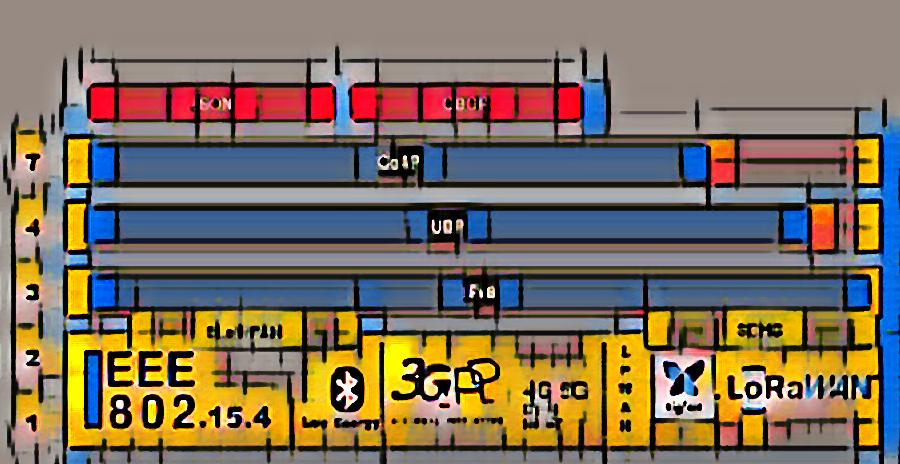
\includegraphics[scale=.70]{Pictures/cover.jpeg}}} % Image background
\centering
\vspace*{5cm}
\par\normalfont\fontsize{35}{35}\sffamily\selectfont
\lgf{\textbf{PROGRAMMER L'INTERNET DES OBJETS }}
\lge{\textbf{PROGRAM THE INTERNET OF THINGS }}
{\LARGE }\par % Book title
\vspace*{1cm}
{\Huge Laurent TOUTAIN}\par % Author name
\endgroup

%----------------------------------------------------------------------------------------
%	COPYRIGHT PAGE
%----------------------------------------------------------------------------------------

\newpage
~\vfill
\thispagestyle{empty}

%\noindent Copyright \copyright\ 2014 Andrea Hidalgo\\ % Copyright notice

\noindent \textsc{IMT Atlantique}\\

\noindent \lgf{Basé sur le \href{https://bit.ly/3Ku0aL8}{MOOC PLIDO}.}\\ % License information
\lge{Based on the  \href{https://bit.ly/3Ku0aL8}{PLIDO MOOC}.} \\
\noindent \textit{\lgf{Publié le \today}\lge{Published \today}} % Printing/edition date

%----------------------------------------------------------------------------------------
%	TABLE OF CONTENTS
%----------------------------------------------------------------------------------------


\chapterimage{pano-tv1.png} % Chapter heading image

\pagestyle{empty} % No headers

\ifthenelse{\boolean{lfrench}}{
\renewcommand\contentsname{Table des Matières}
\renewcommand{\bibname}{Bibliographie}
}{}
\ifthenelse{\boolean{lenglish}}{
\renewcommand\contentsname{Table of Contents}
\renewcommand{\bibname}{Bibliography}
}{}

\cleardoublepage
\tableofcontents% Print the table of contents itself

%\cleardoublepage % Forces the first chapter to start on an odd page so it's on the right

\pagestyle{fancy} % Print headers again

%----------------------------------------------------------------------------------------
%	CHAPTERS
%----------------------------------------------------------------------------------------
\cleardoublepage

\lgf{\chapter*{Acronymes}}
\lge{\chapter*{Acronyms}}

\begin{multicols}{2}
\begin{acronym}
\acro{3GPP}{3rd Generation Partnership Project}
\acro{ABP}{Authentication By Personalisation}
\acro{ADSL}{Asymmetric Digital Subscriber Line}
\acro{AMQP}{Advanced Message Queuing Protocol}
\acro{AS}{Application Server}
\acro{ASCII}{American Standard Code for Information Interchange}
\acro{BLE}{Bluetooth Low Energy}
\acro{CBOR}{Concise Binaire Object Representation}
\acro{CoAP}{Constrained Application Protocol}
\acro{Cosem}{Companion Specification for Energy Management}
\acro{CRC}{Cyclic Redundancy Check}
\acro{CSV}{Comma Separated Values}
\acro{DLMS}{Device Language Message Specification}
\acro{DTT}{Digital Terrestrial Television}
\acro{DR}{Data Rate}
\acro{GSMA}{GSM Association}
\acro{HTML}{HyperText Markup Language}
\acro{HTTP}{HyperText Transport Protocol}
\acro{HTTPS}{HyperText Transport Protocol Secure}
\acro{IANA}{Internet Assigned Numbers Authority}
\acro{IBAN}{International Bank Account Number}
\acro{IEEE}{Institute of Electrical and Electronics Engineers}
\acro{IETF}{Internet Engineering Task Force}
\acro{IoT}{Internet of Things}
\acro{IP}{Internet Protocol}
\acro{IPv4}{Internet Protocol version 4}
\acro{IPv6}{Internet Protocol version 6}
\acro{IPSO}{IP for Smart Objects}
\acro{ITU}{International Telecommunication Union}
\acro{IRI}{International Resource Identifier}
\acro{ISBN}{International Standard Book Number}
\acro{ISO}{International Standardization Organization}
\acro{JMS}{Java Messaging Service}
\acro{JSON}{JavaScript Object Notation}
\acro{JSON-LD}{JavaScript Object Notation  for Linked Data}
\acro{LCIM}{Levels of Conceptual Interoperability Model}
\acro{LPWAN}{Low Power Wide Area Network}
\acro{LwM2M}{Lightweight Machine to Machine}
\acro{LNS}{LoRaWAN Network Server}
\acro{MQTT}{Message Queuing Telemetry Transport}
\acro{NAT}{Network Address Translation}
\acro{NGW}{Network GateWay}
\acro{NIDD}{Non IP Data Delivery}
\acro{OMA}{Open Mobile Alliance}
\acro{OTAA}{Over The Air Authentication}
\acro{OVH}{On Vous Herbèrge}
\acro{PAC}{Porting Authorization Code}
\acro{REST}{REpresentational State Transfer}
\acro{RFC}{Request For Comments}
\acro{RGW}{Radio GateWay}
\acro{RNIPP}{Répertoire National d'Identification des Personnes Physiques}
\acro{RSSI}{Received Signal Strength Indicator}
\acro{RTT}{Round Trip Time}
\acro{SCEF}{Service Capability Exposure Function}
\acro{SenML}{Sensor Measuring List}
\acro{SCHC}{Static Context Header Compression}
\acro{SF}{Spreading Factor}
\acro{SNR}{Signal to Noise Ratio}
\acro{SSID}{Service Set IDentifier}
\acro{STIC}{Sciences et Technologies de l’Information et de la Communication}
\acro{TCP}{Transmission Control Protocol}
\acro{TLV}{Type Length Value}
\acro{TNT}{Télévision Numérique Terrestre}
\acro{TTN}{The Things Network}
\acro{UDP}{User Datagram Protocol}
\acro{UIT}{Union internationale des télécommunications}
\acro{UNB}{Ultra Narrow-Band}
\acro{URI}{Universal Resource Identifier}
\acro{URL}{Univeral Resource Locator}
\acro{URN}{Univeral Resource Name}
\acro{VPS}{Virtual Private Server}
\acro{W3C}{World Wide Web Consortium}
\acro{WWW}{World Wide Web}
\acro{XML}{Extensible Markup Language}
\acro{XMPP}{Extensible Messaging Protocol et Presence}
\end{acronym}
\end{multicols}

%\setboolean{allchap}{true} % true: take all, false take nothing only /input



\Input{Part00-liminaire}
\Input{Part01.0-Intro}
\Input{Part02.0-ArchiIP}
\Input{Part02.5-Wireshark}
\Input{Part03.0-Modbus}
\Input{Part04.0-ArchiIoT}
\Input{Part05.0-Data}
\Input{Part06.0-VSensors}
\cleardoublepage

\lgf{\chapter{Séries temporelles}}
\lge{\chapter{Time series}}


\begin{wrapfigure}{r}{3cm}
\Youtube{https://youtu.be/xrdCY4iN40s}
\end{wrapfigure}

\lgf{Les capteurs virtuels que nous avons programmés jusqu’à présent émettent les données à chaque fois que celles-ci sont mesurées. 
Cela permet au serveur de suivre en temps réel le comportement du système étudié. 
Mais dans certains cas, le temps réel n’est pas nécessaire et il est préférable de limiter le nombre d’émissions, par exemple pour économiser l'énergie du capteur.}
\lge{The virtual sensors that we have programmed so far emit data each time they have a measurement. 
This allows the server to follow the behavior of the studied system in real time. 
But in some cases, real time is not necessary and it is preferable to limit the number of emissions, for example to save the energy of the sensor.}

\lgf{Pour ce faire, nous pouvons utiliser un tableau qui va accumuler les valeurs et l’envoyer quand le tableau atteint une certaine taille.}
\lge{To do this, we can use an array that will accumulate the values and send it when the array reaches a certain size.}


\lgf{\section{Envoi d'un tableau}}
\lge{\section{Sending an array}}


\lgf{Le programme \pprog{minimal\_humidity1.py}{plido-tp3} accumule les données dans un tableau \texttt{h\_humidity} quand celui-ci atteint 30 éléments (ligne 17), les données sont envoyées au serveur.}
\lge{The program \pprog{minimal\_humidity1.py}{plido-tp3} accumulates the data in an array \texttt{humidity} when this one reaches 30 elements (line 17), the data are sent to the server.}

\pythonlst{minimal\_humidity1.py}



\begin{termc}[backgroundcolor=\color{palerod}, basicstyle=\ttfamily\small, escapechar=\#]
1 4 [3241]
2 7 [3241, 2945]
3 10 [3241, 2945, 2762]
4 13 [3241, 2945, 2762, 2625]
5 16 [3241, 2945, 2762, 2625, 2480]
6 19 [3241, 2945, 2762, 2625, 2480, 2769]
\end{termc}

\lgf{Le premier chiffre de la ligne indique le nombre d'éléments et le second la taille dans le codage CBOR. On remarque que l'ajout d'un élément augmente la taille du tableau de 3 octets. Les valeurs correspondant à une mesure d'humidité ne varient pas fortement. Ainsi un tableau de 30 mesures a une taille de 92 octets.}
\lge{The first digit of the line indicates the number of elements and the second the size in the CBOR coding. We notice that adding an element increases the size of the array by 3 bytes. The values corresponding to a moisture measurement do not vary greatly. Thus an array of 30 measurements has a size of 92 bytes.}

\lgf{\section{Codage par différence}}
\lge{\section{Differential coding}}

\lgf{On peut optimiser le volume de données transférées en utilisant un codage par delta (i.e. la variation de l'humidité). 
La première valeur du tableau correspond à la valeur mesurée tandis que les suivantes représentent la différence entre la valeur mesurée et la précédente.}
\lge{The amount of data transferred can be optimized by using delta coding (i.e. the variation in humidity). 
The first value in the table is the measured value while the following values represent the difference between the measured value and the previous one.}

\pythonlst[firstline=17,lastline=26,  firstnumber=17]{minimal\_humidity2.py}%[firstline=282,lastline=19, firstnumber=282]

\lgf{Le programme \pprog{minimal\_humidity2.py}{plido-tp3} gère différemment le remplissage du tableau~:}
\lge{The program \pprog{minimal\_humidity2.py}{plido-tp3} handles the filling of the array differently:}

\begin{itemize}
    \item 
        \lgf{ligne 14 et 15, si le tableau est vide, le tableau est créé avec la valeur mesurée,}
        \lge{line 14 and 15, if the table is empty, the table is created with the measured value,}
    \item 
        \lgf{ligne 16 à 22, sinon si le tableau est plein, il est sérialisé en CBOR et envoyé au serveur, puis réinitialisé avec la valeur mesurée,}
        \lge{line 16 to 22, otherwise if the table is full, it is serialized in CBOR and sent to the server, then reset with the measured value,}
    \item 
        \lgf{ligne 23 et 24, sinon la différence entre la précédente valeur et celle mesurée est stockée dans le tableau.}
        \lge{line 23 and 24, otherwise the difference between the previous value and the measured value is stored in the table.}
\end{itemize}

       \vspace{1em}

\lgf{Le listing suivant donne un exemple d'exécution.}
\lge{The following listing gives an example of execution.}


\begin{termc}[backgroundcolor=\color{palerod}, basicstyle=\ttfamily\small, escapechar=\#]
1 4 [2521]
2 6 [2521, 79]
3 8 [2521, 79, 224]
4 10 [2521, 79, 224, -40]
5 12 [2521, 79, 224, -40, -112]
6 13 [2521, 79, 224, -40, -112, 1]
7 15 [2521, 79, 224, -40, -112, 1, 130]
8 18 [2521, 79, 224, -40, -112, 1, 130, -288]
9 21 [2521, 79, 224, -40, -112, 1, 130, -288, 299]
\end{termc}

\lgf{Ceci met en valeur deux souplesses de CBOR~:}
\lge{This highlights two flexibilities of CBOR:}
\begin{itemize}
    \item 
        \lgf{la taille du tableau est dynamique. Si l’on change le nombre de valeurs à transmettre, le tableau l’indique et l’on n’a pas besoin de modifier le code du récepteur~;}
        \lge{the size of the table is dynamic. If the number of values to be transmitted is changed, the array indicates this and there is no need to modify the receiver code;}
    \item 
        \lgf{la taille des données dépend de leur valeur. 
        Pour les variations entre -24 et +23, un seul octet sera nécessaire. 
        On le voit sur l’exemple précédent : l’ajout de la valeur '1' dans le tableau fait passer la taille de la représentation CBOR de 12 à 135 octets. Les valeurs entre 256 et +255 sont transmises sur 2 octets ; il est donc possible de cette manière d’optimiser la transmission sans ajouter de contrainte. S’il y avait une brusque variation de l’humidité, la représentation CBOR s’adapterait pour la transmettre.}
        \lge{the size of the data depends on its value. 
        For variations between -24 and +23, only one byte will be necessary. 
        We can see it on the previous example: the addition of the value '1' in the table increases the size of the CBOR representation from 12 to 135 bytes. The values between 256 and +255 are transmitted on 2 bytes; it is thus possible in this way to optimize the transmission without adding constraints. If there was a sudden change in humidity, the CBOR representation would adapt to transmit it.}
        
\end{itemize}

\lgf{La taille est réduite d"un tiers (environ 66 octets) pour transmettre la même information.}
\lge{The size is reduced by one third (about 66 bytes) to transmit the same information.}

\section{Architecture}

\lgf{La figure~\vref{fig-client-serveur} représente l'architecture générale du système. Le programme \pprog{minimal\_humidity2.py}{plido-tp3} fournit les séries temporelles. Il reste à définir le programme serveur qui va les traiter et faire appel à un autre service pour les afficher sous forme de graphe. }
\lge{Figure~\vref{fig-client-server} represents the general architecture of the system. The program \pprog{minimal_humidity2.py}{plido-tp3} provides the time series. It remains to define the server program which will process them and call another service to display them in the form of a graph. }


       \vspace{1em}


\lgf{Si l'on suit le flux d'information, le capteur va produire des données au format CBOR pour être compact et le programme serveur va transformer cette information en une structure JSON respectant les spécifications du service d'affichage.}
\lge{If we follow the information flow, the sensor will produce data in CBOR format to be compacted and the server program will transform this information into a JSON structure respecting the specifications of the display service.}

\begin{figure}[tbp]
\centerline{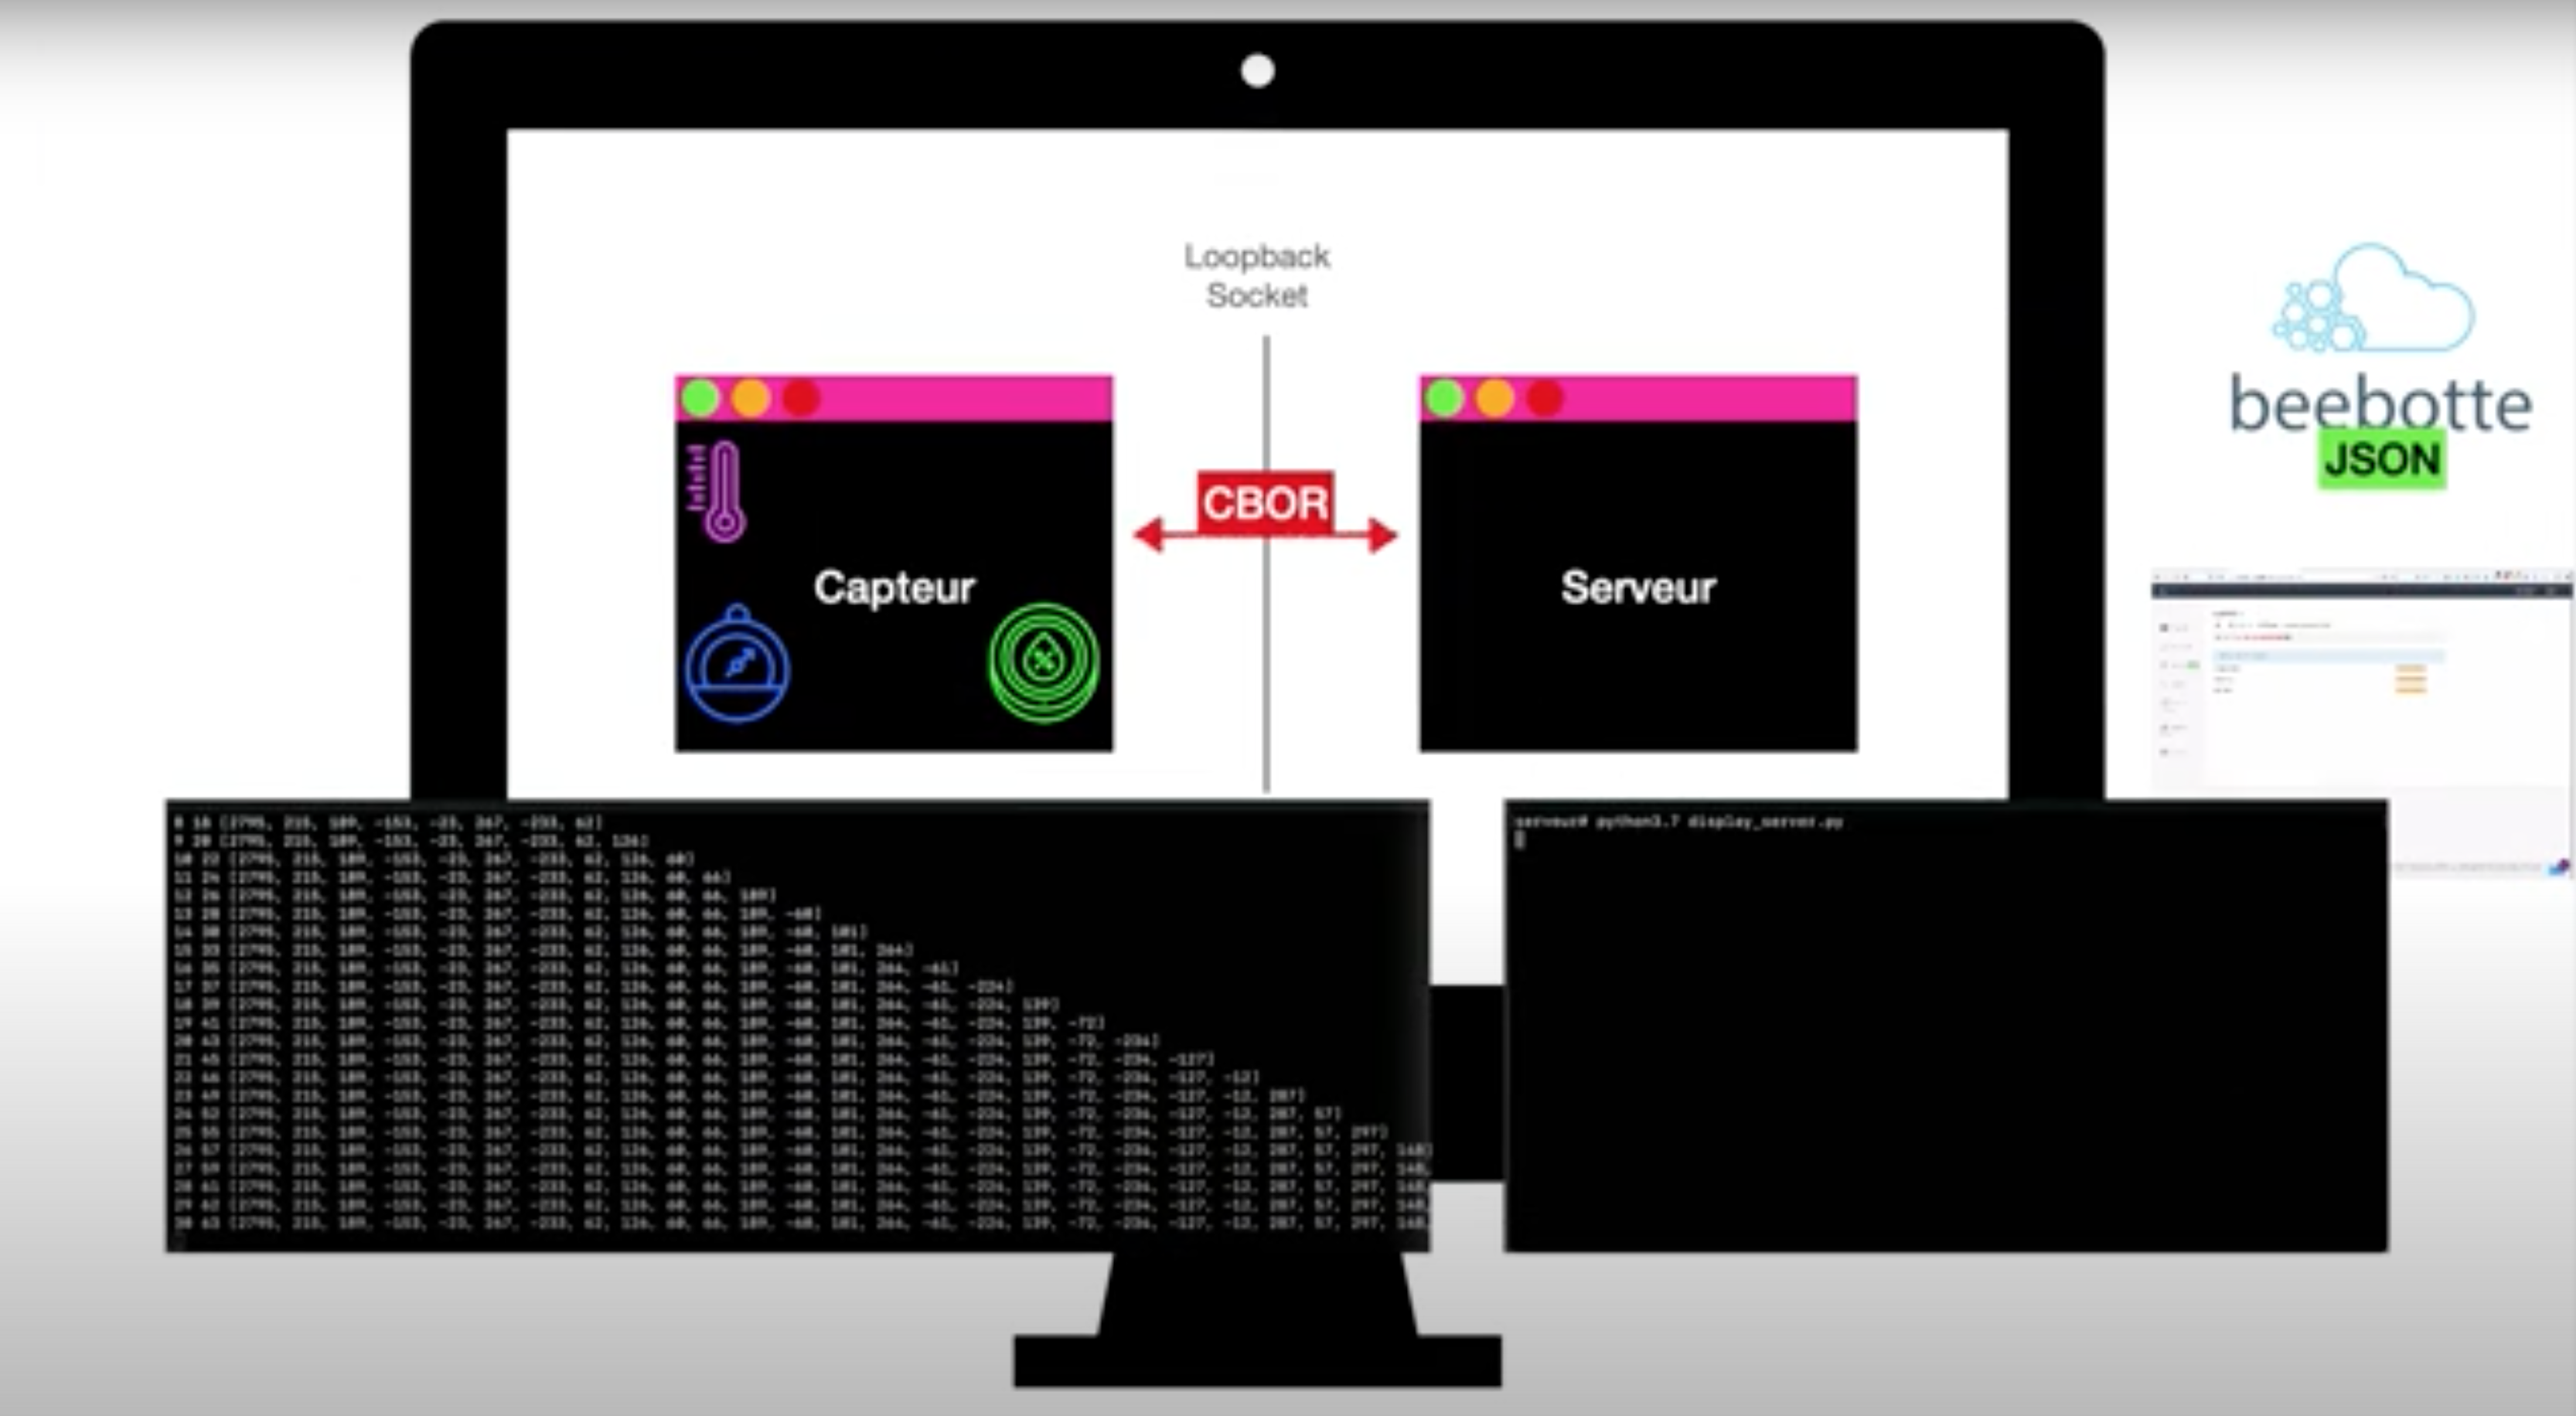
\includegraphics[width=1\columnwidth]{Pictures/Capture40.png}}
\lgf{\caption{Architecture Client/Serveur}}
\lge{\caption{Client/Server Architecture}}
\label{fig-client-serveur}
\end{figure}

\section{\Index{Beebotte}}

\lgf{Il existe plusieurs sites qui permettent de le faire. Nous allons utiliser \url{https://beebotte.com}, mais ce que nous allons présenter peut très bien s'appliquer à d'autres sites.}
\lge{There are several sites that allow you to do this. We are going to use \url{https://beebotte.com}, but what we are going to present can very well be applied to other sites.}

\subsection{Configuration}

\begin{wrapfigure}{r}{3cm}

\includegraphics[width=.2\columnwidth]{Pictures/beebotte.png}
\end{wrapfigure}

\lgf{La première étape consiste à créer un compte en cliquant sur \textit{Sign Up} sur la page de garde et en remplissant un formulaire classique avec votre login, adresse de courrier électronique et mot de passe. Une fois le compte validé, le service est accessible.}
\lge{The first step is to create an account by clicking on \textit{Sign Up} on the front page and filling out a standard form with your login, email address and password. Once the account is validated, the service is accessible.}


\lgf{Le compte nous permet de nous authentifier pour gérer les données sur le site, mais il faut également disposer d’autorisation pour pouvoir y déposer des données via l’\Index{API REST}.
Pour cela, il faut se rendre sur la page \textit{Account Setting} puis l’onglet \textit{Access Management}. 
Cette page (cf. figure~\vref{fig-bb-key}) donne une clé et un secret pour gérer l’ensemble des données sur le site. }
\lge{The account allows us to authenticate ourselves to manage the data on the site, but we also need to have authorization to be able to deposit data via the \Index{API REST}.
To do this, you must go to the \textit{Account Setting} page and then the \textit{Access Management} tab. 
This page (see figure~\vref{fig-bb-key}) gives a key and a secret to manage all the data on the site. }


\begin{figure}[tbp]
\centerline{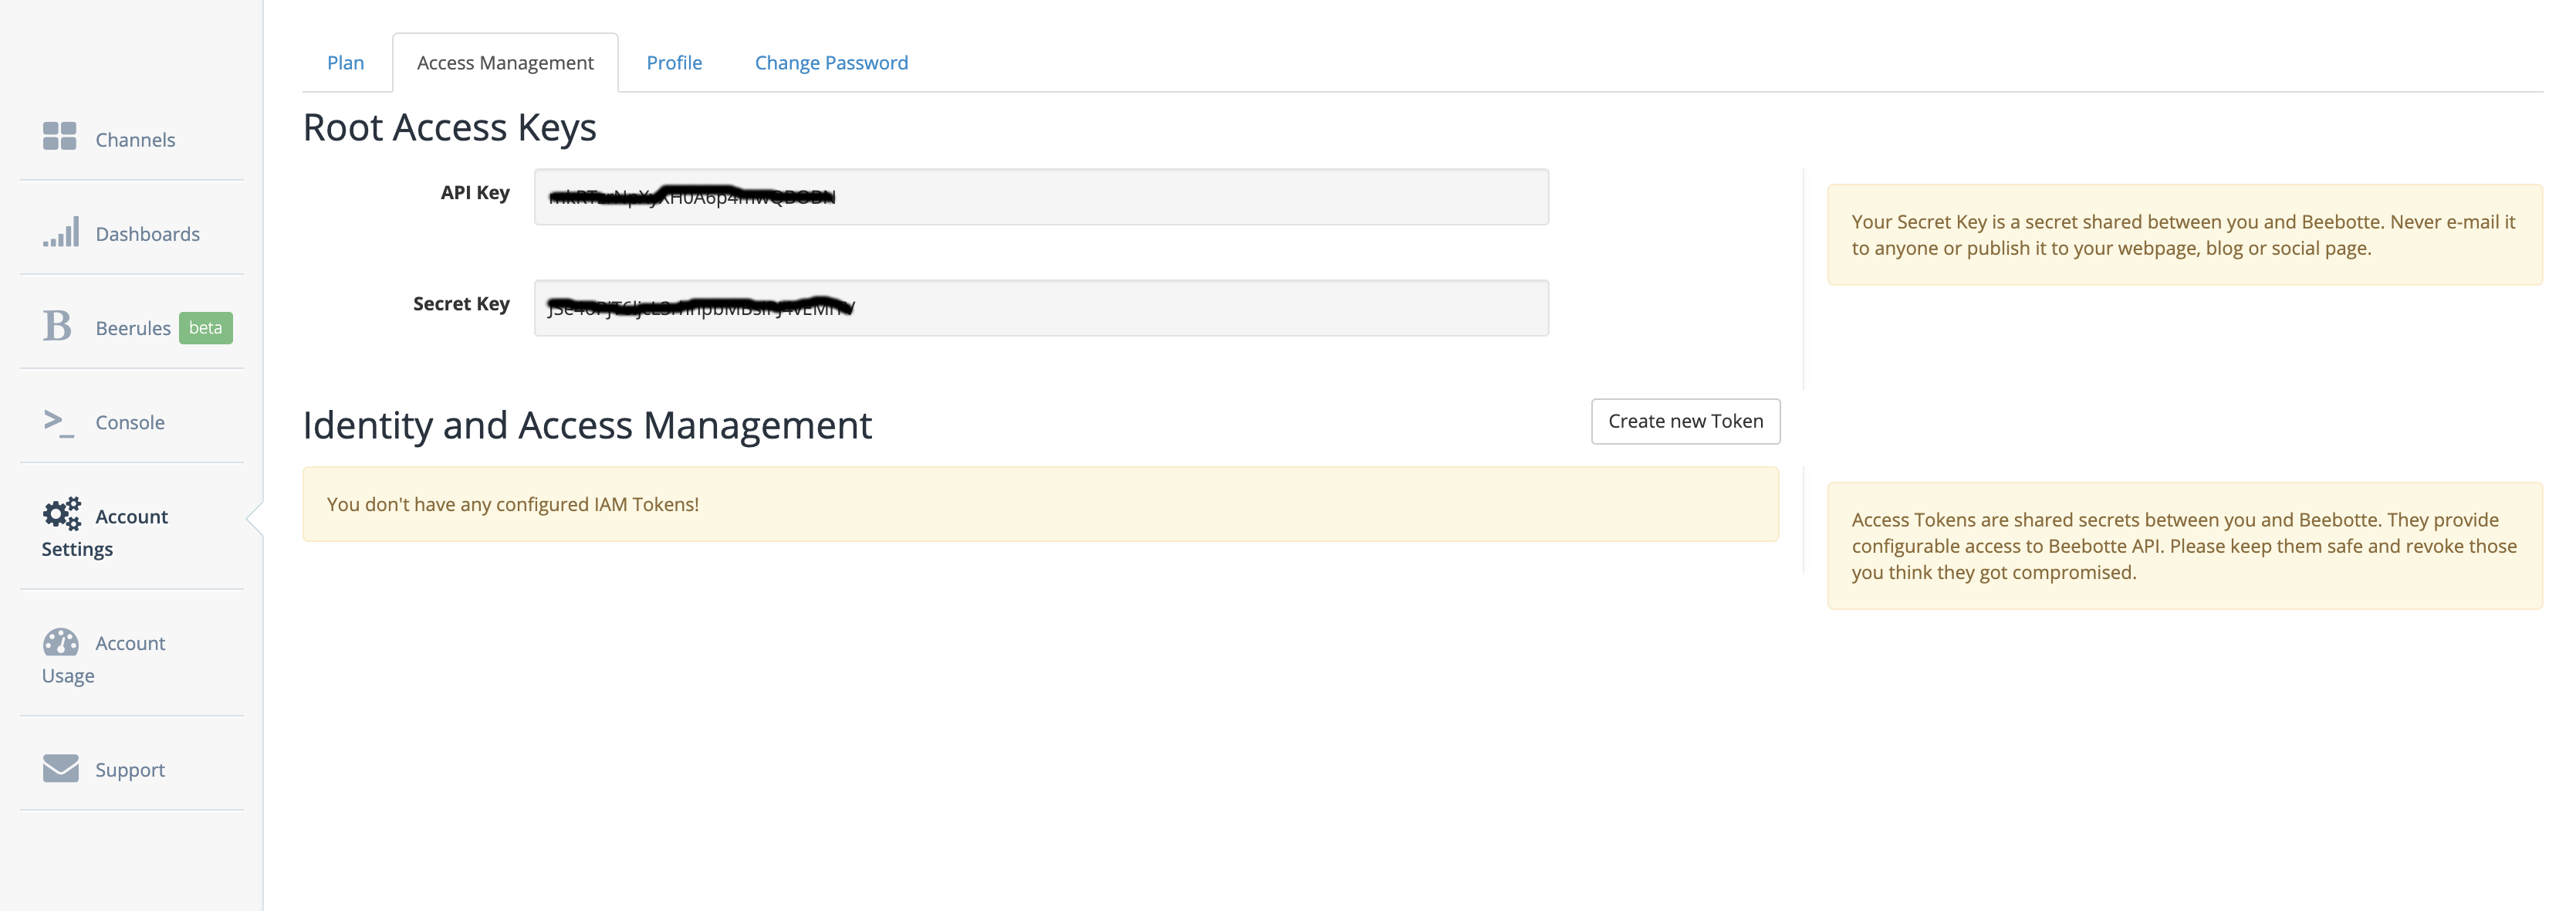
\includegraphics[width=1\columnwidth]{Pictures/bb_root_token.png}}
\lgf{\caption{Clé et secret pour l'authentification}}
\lge{\caption{Key and secret for authentication}}
\label{fig-bb-key}
\end{figure}

\lgf{Notez ces valeurs et stockez les dans un fichier \pprog{config\_bbt.py}{plido-tp3} qui a cet aspect (vos valeurs sont forcément différentes)~:}
\lge{Note these values and store them in a file called \pprog{config\_bbt.py}{plido-tp3} that looks like this (your values are bound to be different):}

\pythonlst{config\_bbt.py}

\lgf{Nous allons maintenant créer un canal (\textit{channel}) dans lequel nous allons définir les objets correspondant aux capteurs. En Cliquant sur \textit {Channels} puis \textit{Create New}, la page représentée figure~\vref{fig-new-channel} apparaît. }
\lge{We are now going to create a channel (\textit{channel}) in which we will define the objects corresponding to the sensors. By clicking on \textit{Channels} and then \textit{Create New}, the page shown in figure~ref{fig-new-channel} appears. }

\lgf{Il faut donner un nom au channel (\textit{capteurs} dans l'exemple), cocher la case \textit{public} et créer trois ressources pour les trois valeurs qui nous intéressent (\textit{temperature}, \textit{humidity}, \textit{presure}) et faire correspondre les unités.}
\lge{You have to give a name to the channel (\textit{sensors} in the example), check the \textit{public} box and create three resources for the three values we are interested in (\textit{temperature}, \textit{humidity}, \textit{presure}) and match the units.}

\lgf{\subsection{Enregistrement des ressources}}
\lge{\subsection{Resource registration}}

\lgf{Le programme \pprog{display\_server.py}{plido-tp3} permet de correspondre avec Beebotte via son API REST. Il commence par l'importation des modules nécessaires~:}
\lge{The program \pprog{display\_server.py}{plido-tp3} allows to correspond with Beebotte via its REST API. It starts by importing the necessary modules:}



\pythonlst[firstline=1,lastline=8, firstnumber=1]{display\_server.py}


\begin{itemize}
    \item 
        \lgf{ligne 4, le module Python \texttt{beebotte}  est disponible pour simplifier la manipulation des données\footnote{S'il n'était pas présent sur votre ordinateur, vous devriez l'installer avec la commande \texttt{pip3 install beebotte}.}.}
        \lge{line 4, the Python module \texttt{beebotte} is available to simplify the manipulation of data\footnote{If it was not present on your computer, you should install it with the command \texttt{pip3 install beebotte}.}.}
    \item 
        \lgf{ligne 5, le module \texttt{contient} la clé et le secret nécessaire à la connexion obtenu précédemment.}
        \lge{line 5, the module \texttt{contains} the key and the secret necessary to the connection obtained previously.}
    
\end{itemize}

\pythonnxt[firstline=9,lastline=11, firstnumber=9]{display\_server.py}

\begin{itemize}
    \item 
        \lgf{ligne 10 et 11 permette d'ouvrir la socket pour communiquer avec les capteurs.}
        \lge{line 10 and 11 allow to open the socket to communicate with the sensors.}
\end{itemize}

\pythonnxt[firstline=12,lastline=14, firstnumber=12]{display\_server.py}

\begin{itemize}
    \item 
        \lgf{ligne 13 une instance permettant la connexion avec les serveurs de Beebotte est définie grâce à la fonction \pfunction{beebotte}{BBT}. Les paramètres de connexion provenant du module \texttt{config\_bbt} sont pris en compte. }
        \lge{line 13 an instance allowing the connection with the Beebotte servers is defined thanks to the function \pfunction{beebotte}{BBT}. The connection parameters from the module \texttt{config\_bbt} are taken into account. }
\end{itemize}

\pythonnxt[firstline=41,lastline=45, firstnumber=41]{display\_server.py}

\lgf{Dans le programme principal, un boucle sans fin attend la série temporelle codée en CBOR venant du capteur (ligne 42), les transforme tableau Python (ligne 44) et appelle la fonction \texttt{to\_btt} en précisant~:}
\lge{In the main program, an endless loop waits for the CBOR coded time series coming from the sensor (line 42), transforms them into a Python array (line 44) and calls the function \texttt{to\_btt} by specifying:}
\begin{itemize}
    \item 
        \lgf{le canal et la ressource qui ont été définie précédemment sur Beebotte~;}
        \lge{the channel and resource that were previously defined on Beebotte;}
    \item 
        \lgf{la série temporelle~;}
        \lge{the time series;}
    \item 
        \lgf{la précision pour transformer ces entiers en flottant.}
        \lge{the precision to transform these integers into floats.}
\end{itemize}

\pythonnxt[firstline=15,lastline=38, firstnumber=15]{display\_server.py}

\lgf{La fonction \texttt{to\_bbt} fait l’essentiel du travail de transformation. Elle prend en argument~:}
\lge{The function \texttt{to\_bbt} does most of the transformation work. It takes as argument:}

\begin{itemize}
    \item 
        \lgf{le nom du canal créé sur Beebotte. Dans notre cas, ce sera \texttt{capteurs}~;}
        \lge{the name of the channel created on Beebotte. In our case, it will be \texttt{sensors};}
    \item  
        \lgf{le nom de l’objet dans ce canal que nous avons également créé sur le site web. Dans notre cas, ce sera \texttt{humidity}~;}
        \lge{the name of the object in this channel that we have also created on the website. In our case, it will be \texttt{humidity};}
    \item  
        \lgf{le tableau Python des mesures codées en delta~;}
        \lge{the Python table of delta-coded measurements;}
    \item  
        \lgf{le facteur multiplicatif, c’est-à-dire la précision. Ici, il faudra diviser par 100~;}
        \lge{the multiplicative factor, i.e. the precision. Here, you will have to divide by 100;}
    \item  
        \lgf{la période entre deux mesures ; cela nous permettra de calculer l’instant de la mesure. Par défaut, la période est de 10 secondes~;}
        \lge{the period between two measurements; this will allow us to calculate the time of the measurement. By default, the period is 10 seconds;}
    \item  
        \lgf{le temps de réception du message pour dater les échantillons. S’il n’est pas spécifié, le temps courant est pris.}
        \lge{the time of reception of the message to date the samples. If it is not specified, the current time is taken.}

\end{itemize}

       \vspace{1em}

\lgf{Cette fonction transforme le tableau Python suivant~:}
\lge{This function transforms the following Python table:}


\begin{termc}[backgroundcolor=\color{palerod},  basicstyle=\ttfamily\small, escapechar=\#]
[3311, 124, -144, -188, -94, 289, -1, -72, 1 ...
\end{termc}
\noindent
\lgf{en un tableau de dictionnaire~:}
\lge{into a dictionary table:}

\begin{termc}[backgroundcolor=\color{palerod},  basicstyle=\ttfamily\small, escapechar=\#]
[{'data': 33.11, 'resource': 'humidity', 'ts': 1596730115000.0},
 {'data': 34.35, 'resource': 'humidity', 'ts': 1596730125000.0},
 {'data': 32.91, 'resource': 'humidity', 'ts': 1596730135000.0},
 {'data': 31.03, 'resource': 'humidity', 'ts': 1596730145000.0},
 ...
\end{termc}

       \vspace{1em}

\lgf{Chaque dictionnaire contient trois éléments imposés par Beebotte :}
\lge{Each dictionary contains three elements imposed by Beebotte:}

\begin{itemize}
    \item 
        \lgf{le nom de la ressource (\texttt{resource}) telle qu'elle a été définie sur l’interface pour le canal~;}
        \lge{the name of the resource (\texttt{resource}) as defined on the interface for the channel;}
    \item 
        \lgf{la valeur associée pour cette ressource (\texttt{data})~;}
        \lge{the associated value for this resource (\texttt{data});}
    \item 
        \lgf{l’instant à laquelle cette mesure a été faite (\texttt{ts}). Le temps est représenté suivant le format \Index{Epoch} qui compte le nombre de secondes depuis le premier Janvier 1970\footnote{voir \url{https://www.epochconverter.com/} pour les conversions.}.}
        \lge{the time at which this measurement was made (\texttt{ts}). The time is represented according to the format \Index{Epoch} which counts the number of seconds since the first of January 1970 \footnote{see \url{https://www.epochconverter.com/} for the conversions}.}
\end{itemize}

       \vspace{1em}

\lgf{Le calcul du \textit{timestamp} (\texttt{ts}) est l’opération la plus complexe de cette fonction mais les module \texttt{time} et \texttt{datetime} facilitent le calcul. 
Si l'argument \texttt{epoch} a été fourni lors de l'appel, la fonction prend cette valeur, sinon le calcule ligne 23. La fonction \pfunction{datetime}{now} retourne la date et l'heure courante, qui est transformé en un tuple grâce à la fonction \pfunction{datetime}{timetuple}. A partir de ce dernier, la fonction \pfunction{time}{maketime} le converti en epoch. }
\lge{The calculation of the \texttit{timestamp} (\texttt{ts}) is the most complex operation of this function but the modules \texttt{time} and \texttt{datetime} facilitate the calculation. 
If the argument \texttt{epoch} has been provided at the time of the call, the function takes this value, otherwise it calculates it on line 23. The function \pfunction{datetime}{now} returns the current date and time, which is transformed into a tuple by the function \pfunction{datetime}{timetuple}. From the latter, the function \pfunction{time}{maketime} converts it into epoch. }

\lgf{Ligne 25, l'epoch à laquelle la première mesure du tableau a été faite est calculé en prenant le temps actuel (cela suppose que l’on néglige le temps de traitement et de transmission) auquel on retranche la durée de la capture, c’est-à-dire comme le nombre d’éléments du tableau multiplié par l’intervalle entre chaque mesure (\texttt{period}). }
\lge{Line 25, the epoch at which the first measurement of the array was made is calculated by taking the current time (this assumes that processing and transmission time are neglected) minus the duration of the capture, i.e. as the number of elements in the array multiplied by the interval between each measurement (\texttt{period}). }

\lgf{Ligne 32 à 34 la structure attendue par Beebotte est construite. le résultat est envoyé, ligne 38, grâce à la fonction \pfunction{beebotte}{writeBulk} qui permet d'envoyer un ensemble de valeurs dans un tableau.}
\lge{Line 32 to 34 the structure expected by Beebotte is built. The result is sent, line 38, thanks to the function \pfunction{beebotte}{writeBulk} which allows to send a set of values in an array.}

       \vspace{1em}

\lgf{On peut vérifier que Beebotte a reçu des données en visualisant le canal capteurs sur l’interface Web. On peut voir sur la  figure~\vref{fig-bb-mesure} que seule la ressource \texttt{humidity} a reçu des données. L’interface affiche la dernière valeur reçue et la date de réception.}
\lge{We can verify that Beebotte has received data by viewing the sensor channel on the web interface. We can see on the figure~\vref{fig-bb-measurement} that only the resource \texttt{humidity} has received data. The interface displays the last value received and the date of reception.}

\begin{figure}[tbp]
\centerline{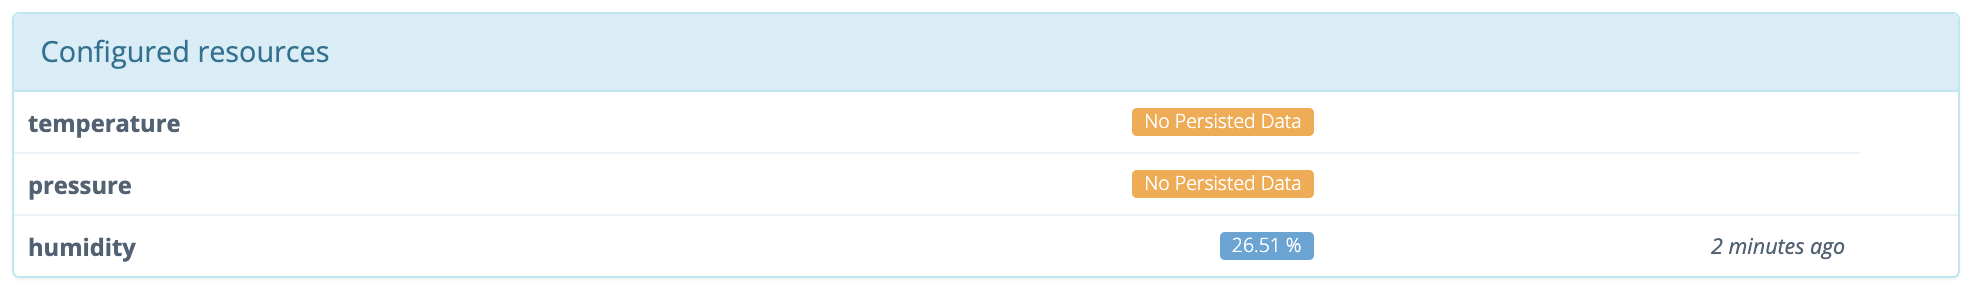
\includegraphics[width=1\columnwidth]{Pictures/bb_mesures.png}}
\lgf{\caption{État des ressources}}
\lge{\caption{Resource status}}
\label{fig-bb-mesure}
\end{figure}

\lgf{\subsection{Visualisation des ressources}}
\lge{\subsection{Resource visualization}}

\lgf{Maintenant que les ressources sont stockées dans les serveurs de Beebotte, il est possible de les visualiser graphiquement, en allant dans \textit{Dashboard} puis \textit{create Dashboard} et \textit {Add Widget} pour sélectionnez un widget comme \textit{Multi-line chart}.}
\lge{Now that the resources are stored in the Beebotte servers, it is possible to visualize them graphically, by going to \textit{Dashboard} and then \textit{create Dashboard} and \textit{Add Widget} to select a widget such as \textit{Multi-line chart}.}

\lgf{Puis, configurez le widget en définissant le canal et la ressource de ce canal comme le montre la figure~\vref{fig-widget}.}
\lge{Then, configure the widget by setting the channel and the resource for that channel as shown in figure~\vref{fig-widget}.}

\begin{figure}[tbp]
\centerline{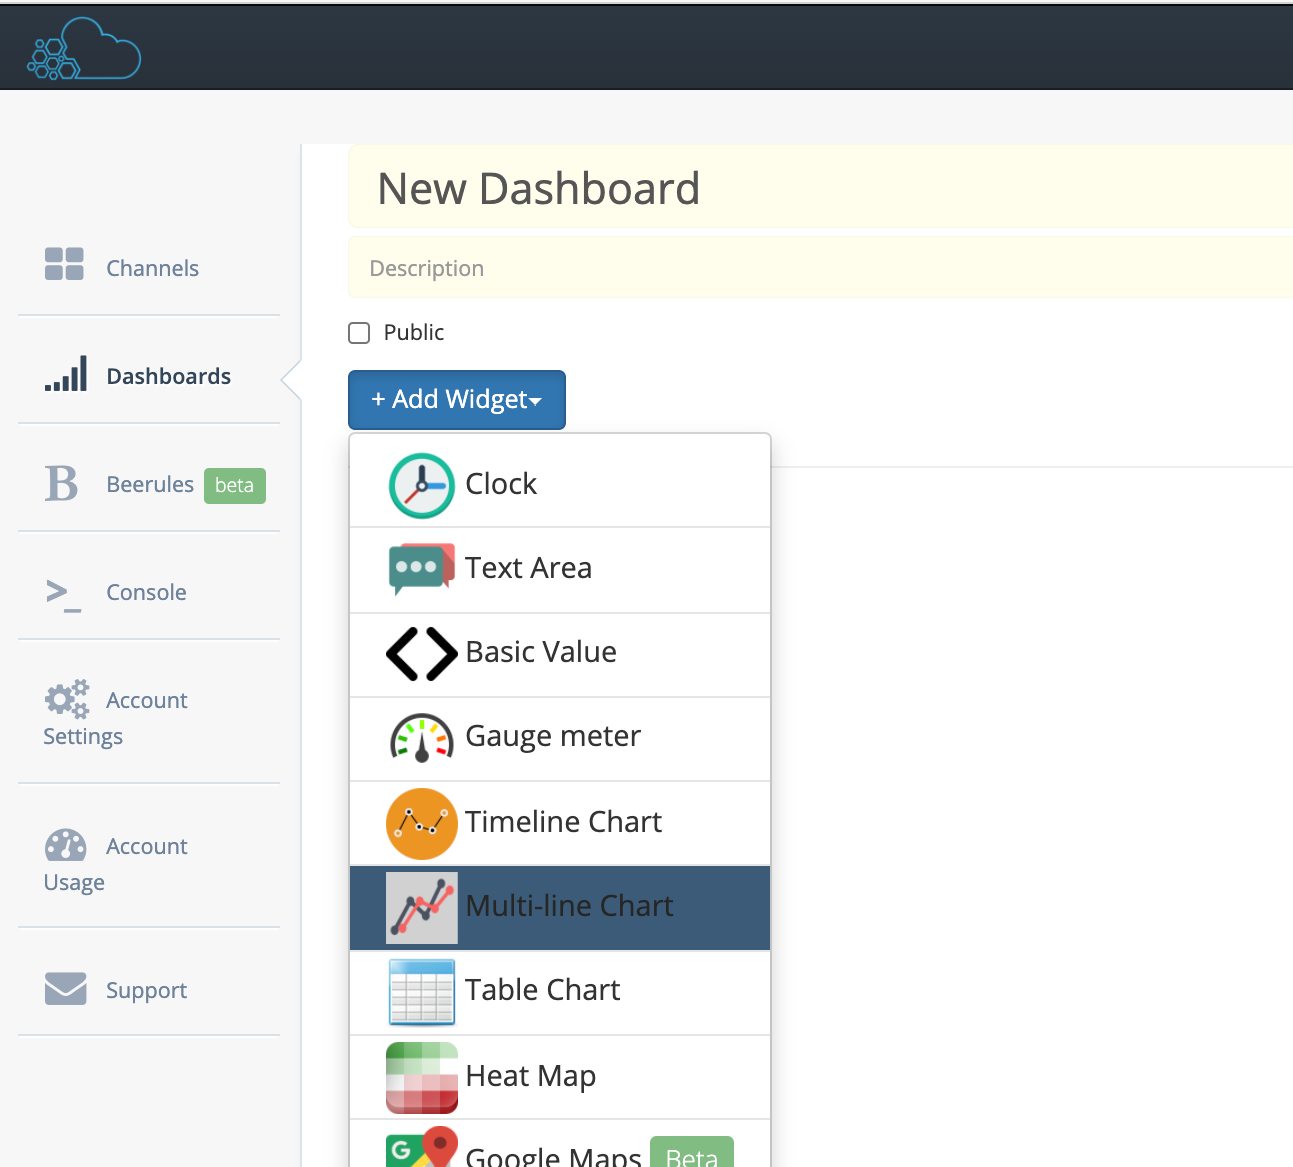
\includegraphics[width=0.5\columnwidth]{Pictures/bb_new_widget.png}}
       \vspace{1em}
\centerline{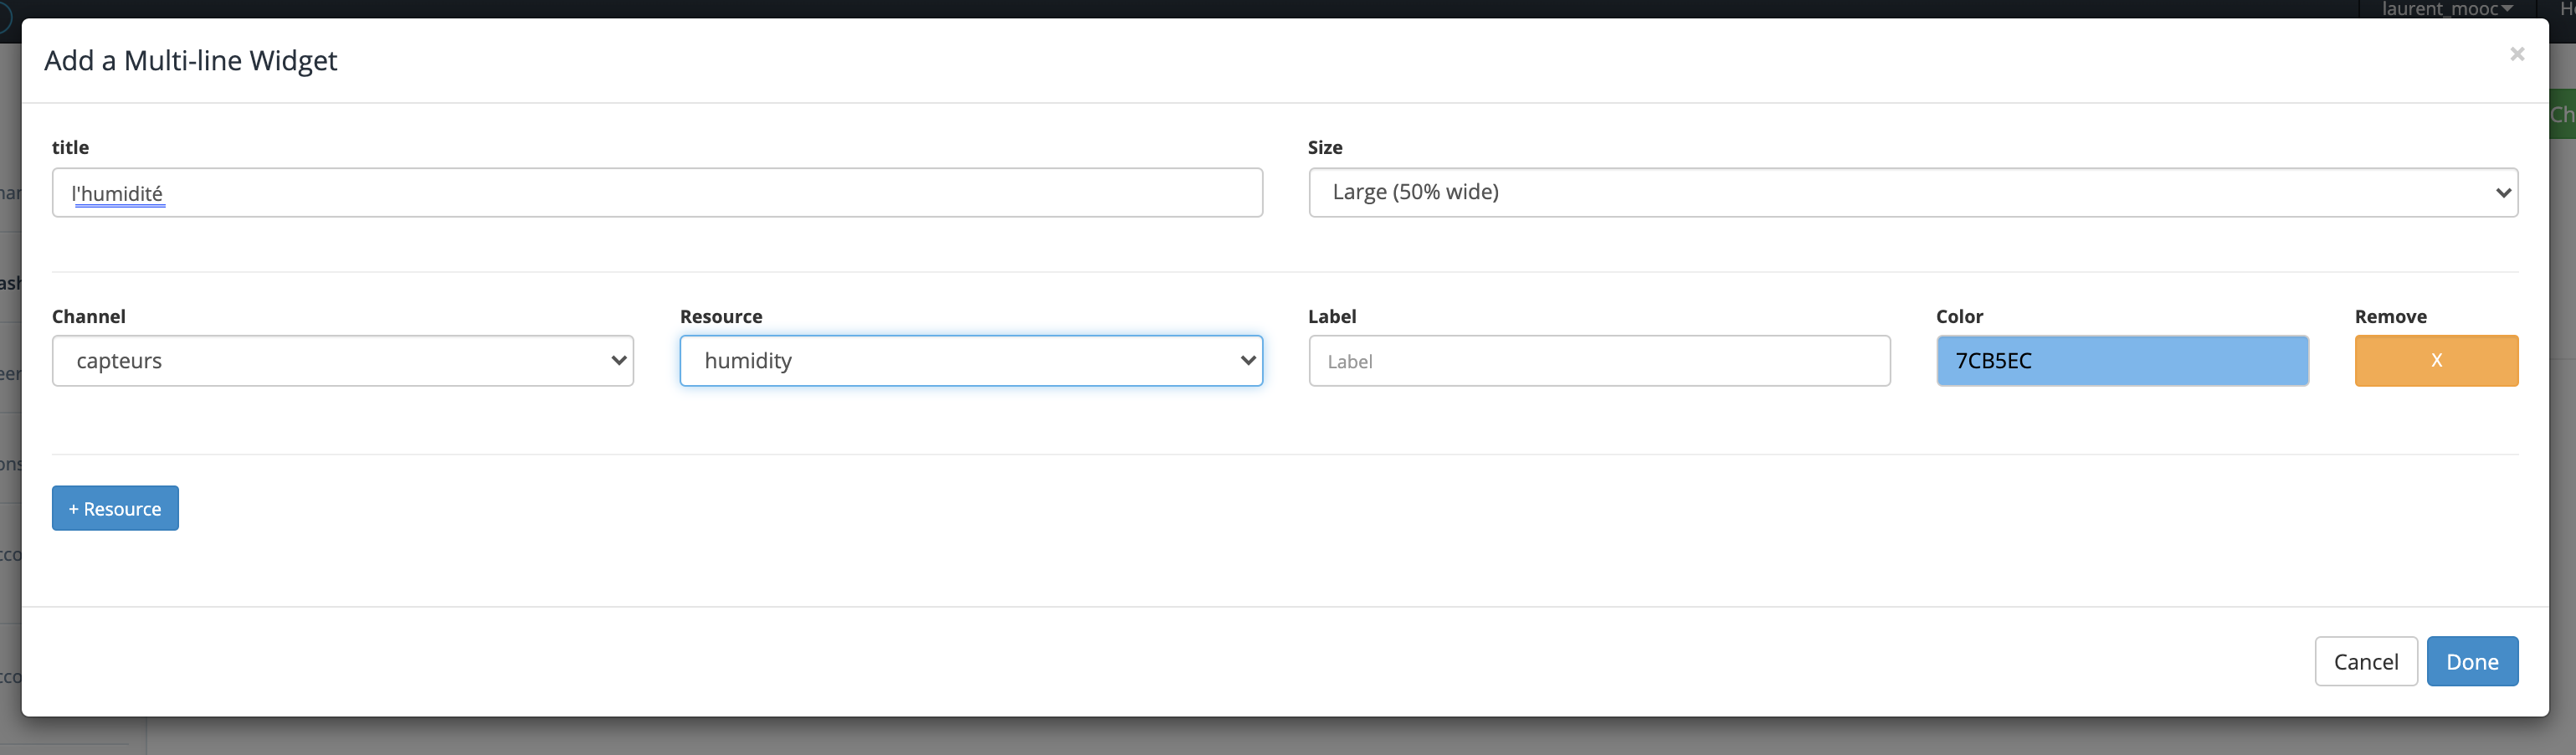
\includegraphics[width=0.5\columnwidth]{Pictures/bb_conf_widget.png}}
\lgf{\caption{Création d'un widget}}
\lge{\caption{Creating a widget}}
\label{fig-widget}
\end{figure}

\lgf{En retournant sur le dashboard, on peut voir l’évolution de l’humidité au cours du temps (cf. figure~\vref{fig-bb-humidity}). }
\lge{By going back to the dashboard, we can see the evolution of the humidity over time (see figure~\vref{fig-bb-humidity}). }

\begin{figure}[tbp]
\centerline{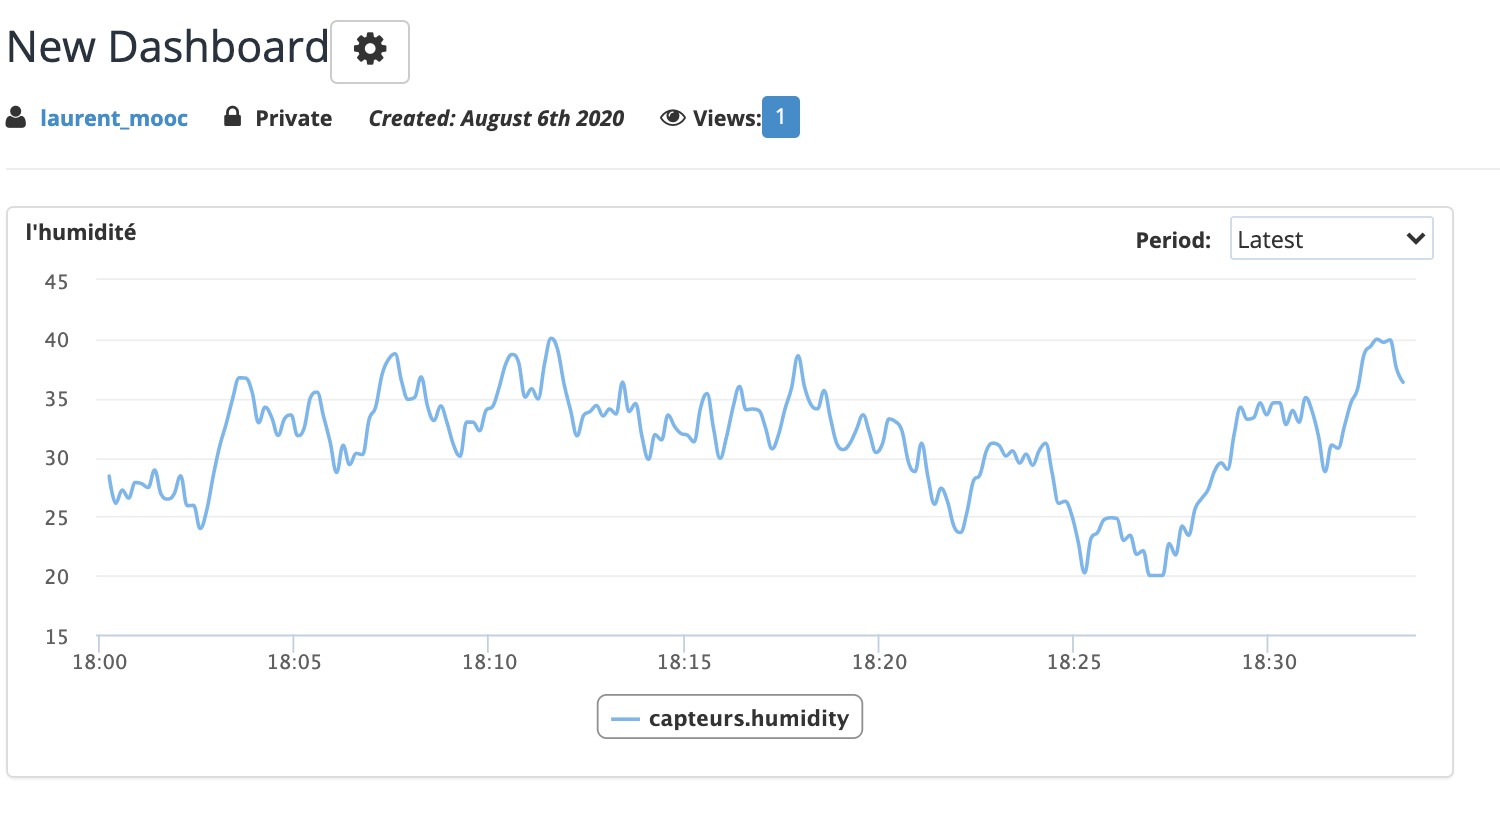
\includegraphics[width=1\columnwidth]{Pictures/bb_humidity.png}}
\lgf{\caption{Suivi de l'humidité}}
\lge{\caption{Humidity monitoring}}
\label{fig-bb-humidity}
\end{figure}

\lgf{\section{Interopérabilité}}
\lge{\section{Interoperability}}

\lgf{La chaîne de collecte de l'information que nous venons de construire allant du capteur à l'affichage, n'est pas complètement interopérable. Certes le capteur envoie des données au format CBOR qui peuvent être interprété par l'autre extrémité, mais le récepteur ne sait pas~:}
\lge{The chain of information collection that we have just built, from the sensor to the display, is not completely interoperable. Certainly the sensor sends data in CBOR format that can be interpreted by the other end, but the receiver does not know:}

\begin{itemize}
    \item 
        \lgf{qu'il s'agit d'une série temporelle codée avec des deltas~;}
        \lgf{that it is a coded time series with deltas;}
    \item  
        \lgf{que les données ont été multipliée par 100 pour pouvoir envoyer des nombres entiers, plus compacts sans perdre trop de précision~;}
        \lgf{that the data have been multiplied by 100 to be able to send whole numbers, more compact without losing too much precision;}
    \item  
        \lgf{que le pas de mesure est de 10 secondes~;}
        \lgf{that the measurement step is 10 seconds;}
    \item  
        \lgf{que les données concernent le taux d'humidité.}
        \lgf{that the data are related to the moisture content.}
\end{itemize}

\lgf{Ces informations ont été précisées dans le programme \pprog{display\_server.py}{plido-tp3}, de même la transformation de la structure de tableau de la série temporelle en un dictionnaire avec des mots clés spécifique à Beebotte on été gravé dans le programme. }
\lge{This information was specified in the program \pprog{display_server.py}{plido-tp3}, as well as the transformation of the table structure of the time series into a dictionary with keywords specific to Beebotte was engraved in the program. }

       \vspace{1em}

\lgf{Nous verrons par la suite comment améliorer cette interopérabilité.}
\lge{We will see later on how to improve this interoperability.}

\lgf{\section{et SenML ?}}
\lge{\section{and SenML?}}

\lgf{Dans la communication avec Beebotte,  le site structure l’envoi des mesures en définissant un dictionnaire JSON avec des mots clés particuliers. Pour utiliser un autre site, le format des échanges doit êter modifié même si les informations restent identiques.}
\lge{In the communication with Beebotte, the site structures the sending of measurements by defining a JSON dictionary with particular keywords. To use another site, the exchange format must be modified even if the information remains identical.}

       \vspace{1em}

\lgf{De plus, lors de la configuration des ressources sur le site de Beebotte, la nature de la mesure a du être précisée~; par exemple, s’il s’agit d’une température, d’un taux d’humidité... Il faut également parfois indiquer le type de la mesure (texte, entier, flottant...) voire les unités. }
\lge{In addition, when configuring the resources on the Beebotte site, the nature of the measurement had to be specified; for example, whether it is a temperature, a humidity level... It is also sometimes necessary to indicate the type of measurement (text, integer, float...) and even the units. }

       \vspace{1em}

\lgf{\ac{SenML} défini dans le \rfc{8428} propose une structuration des données fournie par le capteur. 
Pour réduire l’impact de la transmission, les noms des champs ont été choisis pour être le plus compact possible. 
Par exemple, la lettre \texttt{v}  va indiquer une valeur (à comparer avec la clé \texttt{data} utilisée lors de la communication avec Beebotte). 
Pour être encore plus compact, la représentation en CBOR utilisera des entiers courts au lieu de caractères.}
\lge{\ac{SenML} defined in the \rfc{8428} structures the data provided by the sensor. 
To reduce the impact of the transmission, the field names have been chosen to be as compact as possible. 
For example, the letter \texttt{v} will indicate a value (to be compared with the key \texttt{data} used during the communication with Beebotte). 
To be even more compact, the representation in CBOR will use short integers instead of characters.}

       \vspace{1em}

\lgf{Il est également possible de transporter l’unité de la mesure avec le mot clé \texttt{u} .}
\lge{It is also possible to transport the unit of measurement with the keyword \texttt{u} .}

\lgf{SenML ne définit pas que des unités  du système international, mais également des unités secondaires pour limiter la taille de la représentation. Il sera plus compact de transmettre~:}
\lge{SenML does not only define units of the international system, but also secondary units to limit the size of the representation. It will be more compact to transmit:}

\begin{termc}[backgroundcolor=\color{palerod}, basicstyle=\ttfamily\small, escapechar=\#]
{"u": "MHz", "v": 868}
\end{termc}

\noindent
\lgf{que}
\lge{than}

\begin{termc}[backgroundcolor=\color{palerod},  basicstyle=\ttfamily\small, escapechar=\#]
{"u": Hz", "v": 868000000}.
\end{termc}

\lgf{Le standard définit aussi des temps de base et des valeurs de base auxquelles les temps et les valeurs vont se référer ; ce qui permet également de réduire la taille des valeurs. Finalement, le ou les objets peuvent s’identifier dans les données transmises en définissant un nom de base (\texttt{bn} : \textit{base name}), le nom du capteur (\texttt{n} : \textit{name}) vient compléter le nom de base.}
\lge{The standard also defines base times and base values to which the times and values will refer; this also makes it possible to reduce the size of the values. Finally, the object(s) can be identified in the transmitted data by defining a base name (\texttt{bn} : \textit{base name}), the name of the sensor (\texttt{n} : \textit{name}) completes the base name.}

\lgf{\subsubsection{Émission}}
\lge{\subsubsection{Sending}}

\pythonlst{minimal\_senml\_client.py}

\lgf{Le programme \pprog{minimal\_senml\_client.py}{plido-tp3} illustre le fonctionnement de SenML. Il repose sur deux objets~:}
\lge{The program \pprog{minimal_senml\_client.py}{plido-tp3} illustrates how SenML works. It is based on two objects:}

\begin{itemize}
    \item
        \lgf{l'objet \pfunction{kpn\_senml}{SenmlPack} inclus les informations commune à l'objet, comme le nom de base (ici \texttt{device1} ligne 23) ou la base de temps, ligne 24.}
        \lge{the object \pfunction{kpn\_senml}{SenmlPack} includes information common to the object, such as the base name (here \texttt{device1} line 23) or the time base, line 24.}
    \item 
        \lgf{l'objet \pfunction{kpn\_senml}{SenmlRecord} contient une mesure où l'on peut préciser son nom, son unité et sa valeur (lignes 32, 38 et 44). Le temps est également précisé lignes 35, 41 et 47. Ces enregistrements sont ajoutés à l'objet \texttt{pack}.}
        \lge{the object \pfunction{kpn\_senml}{SenmlRecord} contains a measure where we can specify its name, its unit and its value (lines 32, 38 and 44). The time is also specified on lines 35, 41 and 47. These records are added to the \texttt{pack} object.}
\end{itemize}

\lgf{Le programme récupère les trois valeurs de température, humidité et pression (lignes 27 à 29) en les arrondissant à 2 chiffres après la virgule pour la température et l'humidité et converti la pression, d'hecto Pascal en Pascal puisque c'est l'unité définie par SenML. }
\lge{The program retrieves the three values of temperature, humidity and pressure (lines 27 to 29) by rounding them to 2 digits after the decimal point for temperature and humidity and converts the pressure from hecto Pascal to Pascal since this is the unit defined by SenML. }

\lgf{Les mesures se font toutes les 10 seconde (délais ligne 48) et quand le nombre de mesures défini ligne 13 est atteint, le codage SenML en CBOR est envoyé au serveur. }
\lge{Measurements are made every 10 seconds (delays line 48) and when the number of measurements defined on line 13 is reached, the SenML coding in CBOR is sent to the server. }

       \vspace{1em}

\begin{termc}[backgroundcolor=\color{palerod}, basicstyle=\ttfamily\small, escapechar=\#]
[{'bn': 'device1',
  'bt': 1650463643.0,
  'n': 'temperature',
  't': 0.0,
  'u': 'Cel',
  'v': 20.08},
 {'n': 'humidity', 't': 0.0, 'u': '%RH', 'v': 31.1},
 {'n': 'pressure', 't': 0.0, 'u': 'Pa', 'v': 99920}]
JSON length:  197 bytes
CBOR length:  126 bytes
\end{termc}

\lgf{Ce premier listing montre le premier enregistrement pour les trois grandeurs mesurées. Il s'agit d'un tableau de 3 éléments. Le premier contient les valeurs de bases (ici le nom et l'heure de référence) suivi de la grandeur à mesurer, de son unité et sa valeur. Le deuxième et le troisième éléments, mettent à jours le nom de la grandeur, son unité et sa valeur, les autres informations précédemment définies restent valables.}
\lge{This first listing shows the first record for the three measured quantities. It is a table of 3 elements. The first contains the basic values (here the name and the reference time) followed by the quantity to be measured, its unit and its value. The second and third elements update the name of the quantity, its unit and its value, the other information previously defined remains valid.}


\begin{termc}[backgroundcolor=\color{palerod},  basicstyle=\ttfamily\small, escapechar=@]
[@\textcolor{gray}{\{'bn': 'device1',}@
 @\textcolor{gray}{ 'bt': 1650463643.0,}@
 @\textcolor{gray}{ 'n': 'temperature',}@
 @\textcolor{gray}{ 't': 0.0,}@
 @\textcolor{gray}{ 'u': 'Cel',}@
 @\textcolor{gray}{ 'v': 20.08\},}@
 @\textcolor{gray}{\{'n': 'humidity', 't': 0.0, 'u': '\%RH', 'v': 31.1\},}@
 @\textcolor{gray}{\{'n': 'pressure', 't': 0.0, 'u': 'Pa', 'v': 99920},\}@
 {'n': 'temperature', 't': 10.0, 'u': 'Cel', 'v': 20.04},
 {'n': 'humidity', 't': 10.0, 'u': '%RH', 'v': 31.49},
 {'n': 'pressure', 't': 10.0, 'u': 'Pa', 'v': 99872}]
JSON length:  361 bytes
CBOR length:  232 bytes
 \end{termc}
 
 \lgf{Quand on ajoute 10 secondes plus tard de nouvelles mesures,  un temps relatif de 10 secondes est indiqué pour l'enregistrement des températures et il reste valable pour les enregistrements suivants.}
 \lge{When new measurements are added 10 seconds later, a relative time of 10 seconds is indicated for the temperature recording and it remains valid for the following recordings.}
 
 
 \Question{\lgf{Codage}\lge{Encoding}}
 {
 \lgf{A quoi correspond la clé \texttt{\{'u' : 'Cel'\}} que l'on retrouve dans la structure précédente ? }
 \lge{What does the key \texttt{\{'u' : 'Cel'\}} found in the previous structure correspond to? }
 }
 {
 \lgf{ Unité = degrés Celcius}
 \lge{ Unit = degrees Celcius}
 
 }
 
 \Question{\lgf{Accroissement}\lge{Growth}}
 {
 \lgf{Dans les deux représentations JSON et CBOR, de combien la taille est-elle accrue par l'ajout des mesures effectuées ? d'où viennent ces différences ?}
 \lge{In both JSON and CBOR representations, how much is the size increased by adding the measurements made? Where do these differences come from?}
 }
 {
 \lgf{Si l'on regarde le listing précédent, l'ajout des trois mesures fait augmenter la taille de 164 octets pour JSON et 106 pour CBOR. La différence vient de l'utilisation de nombre plus que de chaînes de caractères pour les clés. Ainsi 't' demande 3 caractères en JSON avec les guillemets, codé en CBOR, il faudrait 2 octets, un nombre inférieur à 23 se code sur un seul octet. Il y a egalement les virgules, espaces et fermeture de crochets qui ne sont pas présent en CBOR. Les nombres flottant comme \texttt{19.98} ont une représentation plus compacte en JSON (5 octets) qu'en CBOR où ils consomment 9 octets. Dans tous les cas l'accroissement est fortement dépendant du nom des éléments. Ici, il faut répéter à chaque fois \texttt{temperature}, \texttt{humidity} et \texttt{pressure}, soit 26 caractères.}
 \lge{If we look at the previous listing, adding the three measures increases the size by 164 bytes for JSON and 106 for CBOR. The difference comes from the use of numbers rather than strings for the keys. Thus 't' requires 3 characters in JSON with the quotes, encoded in CBOR, it would take 2 bytes, a number less than 23 is encoded on a single byte. There are also commas, spaces and closing brackets which are not present in CBOR. The floating numbers like \texttt{19.98} have a more compact representation in JSON (5 bytes) than in CBOR where they consume 9 bytes. In all cases the increase is strongly dependent on the name of the elements. Here, it is necessary to repeat each time \texttt{temperature}, \texttt{humidity} and \texttt{pressure}, that is 26 characters.}
 }
 
 \Question {\lgf{Une seule grandeur}\lge{A single value}}
 {
 \lgf{Si on ne s'intéressait qu'à une seule grandeur, par exemple l'humidité. A quoi ressemblerait la structure SenML en JSON ?}
 \lge{If we were only interested in one quantity, for example humidity. What would the SenML structure look like in JSON?}
 }
 {
 \lgf{Chaque nouvelle entrée ajoute 35 octets à la structure~: }
 \lge{Each new entry adds 35 bytes to the structure~: }
 
 \noindent
 [\{'bn': 'device1',  'bt': 1640110457.0, 'n': 'humidty', 'u': '\%RH', 'v': 28.46\},\\
 \{'t': 10.0, 'v': 26.86\},\\
 \{'t': 20.0, 'v': 26.96\},\\
 \{'t': 30.0, 'v': 27.01\}]\\
 }
 
 \lgf{\subsubsection{Réception}}
 \lge{\subsubsection{Receiving}}
 
 \lgf{Le traitement par le module SenML tel qu'il est mis en œuvre n'est pas complet, il ne gère pas correctement les timestamps. Mais, il n'est pas vraiment nécessaire pour traiter ces messages. En effet, comme on l'a vu précédemment, les valeurs SenML sont composés d'une base et d'une valeur. En concaténant les différents éléments du tableau, on garde les clés de base et on remplace les clés qui se répètent à chaque éléments. Cela permet d'avoir une mise en \oe{}uvre très simple du décodage, pour la série SenML qui nous est fournie.}
 \lge{The processing by the SenML module as implemented is not complete, it does not handle timestamps correctly. But, it is not really necessary to process these messages. Indeed, as we have seen previously, SenML values are composed of a base and a value. By concatenating the different elements of the array, we keep the base keys and we replace the keys which are repeated at each element. This allows to have a very simple implementation of the decoding, for the SenML series which is provided to us.}
 
 
 \pythonlst{minimal\_senml\_server.py}
 
 \lgf{Le programme \pprog{minimal\_senml\_server.py}{plido-tp3} va convertir le format SenML codé en CBOR dans le format attendu par Beebotte. 
 La version CBOR utilise des nombres plutôt que des tags.
 Le dictionnaire \texttt{naming\_map} defini lignes 10 à 12 permet la correspondance utilisé par la suite pour rendre le code plus lisible.}
 \lge{The program \pprog{minimal\_senml\_server.py}{plido-tp3} will convert the SenML format encoded in CBOR into the format expected by Beebotte. 
 The CBOR version uses numbers rather than tags.
 The dictionary \texttt{naming\_map} defined on lines 10 to 12 allows the correspondence used afterwards to make the code more readable.}
 
 \lgf{Les lignes 14 à 17 initialisent les communications venant du capteur et celles allant à Beebotte. }
 \lge{Lines 14 to 17 initialize the communications coming from the sensor and those going to Beebotte. }
 
\lgf{Les données reçues ligne 21 sont transformée en structure Python ligne 23. Cette correspondance est possible car Python autorise des clés numériques et celles-ci ne sont pas répétées plusieurs fois dans une map CBOR.}
\lge{The data received on line 21 is transformed into a Python structure on line 23. This correspondence is possible because Python allows numerical keys and these are not repeated several times in a CBOR map.}
 
\lgf{La boucle commençant ligne 28 permet d'explorer tous les éléments du tableau SenML, les nouvelles entrées sont fusionnées avec les anciennes (ligne 29)\footnote{Dans les version plus récentes de Python, il est possible d'utiliser l'opérateur \texttt{|}.}. }
\lge{The loop starting on line 28 allows you to explore all the elements of the SenML array, the new entries are merged with the old ones (line 29)\footnote{ In more recent versions of Python, it is possible to use the \texttt{|} operator.} }

\lgf{Les informations concernant le temps sont ensuite recherchées. 
D'abord le temps (ligne 32) et s'il un temps de base existe (ligne 33) il est ajouté. On procède de même pour la valeur (lignes 38 à 40). Pour le nom, il n'y a pas de concaténation car le nom de base sera utilisé comme canal Beebotte, il est récupéré à la fin ligne 46.}
\lge{The information about the time is then searched for. 
First the time (line 32) and if there is a basic time (line 33) it is added. The same procedure is followed for the value (lines 38 to 40). For the name, there is no concatenation because the basic name will be used as a Beebotte channel, it is recovered at the end of line 46.}

\lgf{A partir de ces informations, la structure attendue par Beebotte est construite ligne 43 en ajoutant le dictionnaire dans le tableau \texttt{bbt\_record}.}
\lge{From this information, the structure expected by Beebotte is constructed line 43 by adding the dictionary in the table \texttt{bbt\_record}.}

\lgf{Ligne 47, l'information est envoyée à Beebotte. Si les clés d'authentification, le nom du canal et des ressources sont correct, les information s'affiche sur le site, comme précédemment. }
\lge{Line 47, the information is sent to Beebotte. If the authentication keys, channel name and resources are correct, the information is displayed on the site, as before. }

\begin{termc}[backgroundcolor=\color{palerod},  basicstyle=\ttfamily\tiny, escapechar=@]
{0: 'temperature', 2: 19.94, 6: 0.0, 1: 'Cel', -2: 'device1', -3: 1650463732.0}
{0: 'humidity', 2: 27.7, 6: 0.0, 1: '%RH', -2: 'device1', -3: 1650463732.0}
{0: 'pressure', 2: 100109, 6: 0.0, 1: 'Pa', -2: 'device1', -3: 1650463732.0}
{0: 'temperature', 2: 19.88, 6: 10.0, 1: 'Cel', -2: 'device1', -3: 1650463732.0}
{0: 'humidity', 2: 24.82, 6: 10.0, 1: '%RH', -2: 'device1', -3: 1650463732.0}
{0: 'pressure', 2: 100056, 6: 10.0, 1: 'Pa', -2: 'device1', -3: 1650463732.0}
{0: 'temperature', 2: 19.93, 6: 20.0, 1: 'Cel', -2: 'device1', -3: 1650463732.0}
{0: 'humidity', 2: 23.74, 6: 20.0, 1: '%RH', -2: 'device1', -3: 1650463732.0}
{0: 'pressure', 2: 100123, 6: 20.0, 1: 'Pa', -2: 'device1', -3: 1650463732.0}
{0: 'temperature', 2: 19.92, 6: 30.0, 1: 'Cel', -2: 'device1', -3: 1650463732.0}
{0: 'humidity', 2: 25.82, 6: 30.0, 1: '%RH', -2: 'device1', -3: 1650463732.0}
{0: 'pressure', 2: 100220, 6: 30.0, 1: 'Pa', -2: 'device1', -3: 1650463732.0}
{0: 'temperature', 2: 19.9, 6: 40.0, 1: 'Cel', -2: 'device1', -3: 1650463732.0}
{0: 'humidity', 2: 24.47, 6: 40.0, 1: '%RH', -2: 'device1', -3: 1650463732.0}
{0: 'pressure', 2: 100173, 6: 40.0, 1: 'Pa', -2: 'device1', -3: 1650463732.0}
[{'data': 19.94, 'resource': 'temperature', 'ts': 1650463732000.0},
 {'data': 27.7, 'resource': 'humidity', 'ts': 1650463732000.0},
 {'data': 100109, 'resource': 'pressure', 'ts': 1650463732000.0},
 {'data': 19.88, 'resource': 'temperature', 'ts': 1650463742000.0},
 {'data': 24.82, 'resource': 'humidity', 'ts': 1650463742000.0},
 {'data': 100056, 'resource': 'pressure', 'ts': 1650463742000.0},
 {'data': 19.93, 'resource': 'temperature', 'ts': 1650463752000.0},
 {'data': 23.74, 'resource': 'humidity', 'ts': 1650463752000.0},
 {'data': 100123, 'resource': 'pressure', 'ts': 1650463752000.0},
 {'data': 19.92, 'resource': 'temperature', 'ts': 1650463762000.0},
 {'data': 25.82, 'resource': 'humidity', 'ts': 1650463762000.0},
 {'data': 100220, 'resource': 'pressure', 'ts': 1650463762000.0},
 {'data': 19.9, 'resource': 'temperature', 'ts': 1650463772000.0},
 {'data': 24.47, 'resource': 'humidity', 'ts': 1650463772000.0},
 {'data': 100173, 'resource': 'pressure', 'ts': 1650463772000.0}]

 \end{termc}
 
 \lgf{Le listing précédent montre cette transformation.
 Les premières lignes correspondent aux enregistrements fusionnées et le tableau final, ce qui a été envoyé à Beebotte.}
 \lge{The previous listing shows this transformation.
 The first rows are the merged records and the final table is what was sent to Beebotte.}
 
 
 \Question{base value}
 {
 \lgf{Pourrait-on utiliser le champ SenML \textit{base value} pour diminuer la taille des données de pression atmosphérique~?}
 \lge{Could we use the SenML field \textit{base value} to decrease the size of the air pressure data~?}
 }
 {
\lgf{Cela serait possible, si cette ressource était envoyée seule.}
\lge{This would be possible, if this resource was sent alone.}
 }
\Input{Part07.0-LoPy}
\Input{Part08.0-Sigfox}
\Input{Part09.0-LoRaWAN}
\Input{Part10.0-CoAP}
\Input{Part10.5-aiocoap}
\Input{Part11.0-LwM2M}






%%%%%%%%%%%%%%%%%%%%%%%%%%%%%%%%%%%%%



\immediate\closeout\tempfile
\setboolean{Response}{false}

\cleardoublepage
\lgf{\chapter{Réponses aux questions}}
\lge{\chapter{Answers to the questions}}
\input{questions}

\cleardoublepage
\printindex

\cleardoublepage
\printbibliography

\end{document}